\documentclass{statsoc}
\usepackage[a4paper]{geometry}
\usepackage{graphicx,psfrag,epsf}
\usepackage{enumerate}
\usepackage{natbib}
\usepackage{amsfonts}
%\let\proof\relax
%\let\endproof\relax
\usepackage{amsmath}
\usepackage{float}
%\usepackage{amsthm}
\usepackage{xcolor}
%\usepackage{amssymb,mathabx}
\usepackage{algorithm, algpseudocode}
%\usepackage[utf8]{inputenc}
\usepackage[english]{babel}
\newtheorem{theorem}{Theorem}
\newtheorem{corollary}{Corollary}%[theorem]
\newtheorem{assumption}{Assumption}
\newtheorem{lemma}[theorem]{Lemma}
%\theoremstyle{definition}
\newtheorem{definition}{Definition}%[section]
\newtheorem{proposition}[theorem]{Proposition}
%\newcommand{\blind}{0}
\title[Efficient MCMC for parameter inference for MJPs]{\bf Efficient MCMC for parameter inference for Markov jump processes}
\author{Boqian Zhang and Vinayak Rao}
\address{Department of Statistics, Purdue University, USA
}
\email{zhan1977@purdue.edu, varao@purdue.edu}
\input{mymacros.tex}

\begin{document}
\def\spacingset#1{\renewcommand{\baselinestretch}
{#1}\small\normalsize} \spacingset{1}


%%%%%%%%%%%%%%%%%%%%%%%%%%%%%%%%%%%%%%%%%%%%%%%%%%%%%%%%%%%%%%%%%%%%%%%%%%%%%%

\begin{abstract}
Markov jump processes (MJPs) are continuous-time stochastic processes 
widely applied in a variety of disciplines. Inference for MJPs typically
proceeds via Markov chain Monte Carlo, the state-of-the-art being an auxiliary
variable Gibbs sampler proposed in~\cite{RaoTeh13}. This algorithm was
designed for the situation where the MJP parameters are known, and Bayesian
inference over unknown parameters is typically carried out by incorporating
this into a larger Gibbs sampler.
%In many situations, the MJP trajectory and parameters can exhibit
%strong coupling, and
This strategy of alternately sampling parameters given path, and
then path given parameters can result in poor Markov chain mixing. In this
work, we propose a simple and elegant algorithm to address this
problem. Our scheme brings Metropolis-Hastings approaches
for discrete-time hidden Markov models to the continuous-time
setting, %and also also ties up some of the loose ends in~\cite{RaoTeh13}. 
resulting in %is
 a complete and clean recipe for
parameter and path inference in MJPs. In our experiments, we
demonstrate superior performance over the Gibbs sampling approach, as well as
another popular approach, particle MCMC~\cite{Andrieu10}.
\end{abstract}
\noindent%
{\it Keywords:}  Markov jump process, Markov chain Monte Carlo, Metropolis-Hasting, Bayesian
inference, Uniformization
%\spacingset{1.45}
\vspace{-.05in}

\section{Introduction}
\label{sec:intro}
Markov jump processes (MJPs) are continuous-time stochastic processes that
have found wide application in fields like computational chemistry~\cite{gillespie97}, 
population genetics~\cite{FearnSher2006}, mathematical finance~\cite{Elliott06}, 
queuing theory~\cite{Breuer2003}, artificial intelligence~\cite{XuShe10} and
social-network analysis~\cite{pan2016markov}. %The references above have
MJPs have been used to model the state of a chemical reaction, the state 
of a queuing network, segmentation of a strand of DNA, user activity on social 
media, among many others.

MJPs model temporal evolution in continuous-time, resulting in 
realistic, mechanistic, and interpretable models. %, often amenable to mathematical analysis. 
These same dynamics however raise computational
challenges in statistical applications, where given partial and noisy 
measurements, one has to make inferences over the latent MJP 
trajectory as well as any system parameters. Such
inference is complicated by two facts: one cannot {\em a priori} 
bound the number of state transitions, and the state-transition times themselves
are continuous-valued. This is in contrast to the situation with
{\em discrete-time} hidden Markov models. %and trajectory inference for 
%MJPs typically proceeds via Markov chain Monte Carlo. 
The state-of-the-art inference method for MJPs is an auxiliary variable Gibbs sampler proposed 
in~\cite{RaoTeh13}, we will henceforth refer to this as the {\algname} 
algorithm. The {\algname} algorithm was designed to sample paths when the MJP parameters
are known. Parameter inference is typically carried out by 
incorporating it into an outer Gibbs sampler that also simulates
parameters given the currently sampled trajectory. 

In many situations, the MJP trajectory and parameters can exhibit 
strong coupling, so that a Gibbs sampler that alternately samples path given
parameters, and then parameters given path can mix poorly.  
In this work, we propose a Metropolis-Hastings framework to address
this issue. Our proposed solution is simple and elegant, additionally,
it ties up some of the loose ends in the Rao-Teh algorithm.
In our experiments, we demonstrate superior 
performance over Gibbs sampling, as well as other approaches like 
particle Markov chain Monte Carlo~\cite{Andrieu10}.

\section{Markov jump processes (MJPs)} 
Formally, a Markov jump process~\cite{Cinlar1975} is a right-continuous 
piecewise-constant stochastic process $S(t)$ taking values in a countable, and 
usually finite state space $\cS$ (see Figure~\ref{fig:naive_mh}, top-left).
For simplicity, we will assume $N$-states, with $\cS = \{1,\ldots,N\}$. Then, 
an MJP is parameterized by two quantities, an $N$-component probability vector 
$\pi_0$ and a rate-matrix $A$. The former gives the distribution over states at 
the initial time (which without loss of generality we assume is $0$), while 
the latter is an $N \times N$-matrix governing the dynamics of the system.  An 
off-diagonal element $A_{ij}$, for some $i \neq j$ gives the rate at 
which the system transitions from state $i$ to $j$. We write $A_i$ for the 
negative of the $i$th diagonal element $A_{ii}$. For an MJP,
$A_i = -A_{ii} = \sum_{j \neq i} A_{ij}$, so that the rows of $A$ sum to $0$.  
$A_i$ gives the total rate at which the system leaves state $i$ for any other state.
To simulate an MJP trajectory over an interval $[0,\cT]$, one follows 
Gillespie's algorithm~\cite{gillespie97}: 
first sample an initial state $s_0$ from the distribution $\pi$, and
then defining $t_0 = t_{curr} = 0$ and $k = 0$, repeat the following two steps while
$t_{curr} < \cT$:
\begin{itemize}
  \item Sample a wait-time $\Delta t_k$ from an exponential distribution with rate 
    $A_{s_k}$.  Set $t_{k+1} = t_{curr} = t_{k} + \Delta t_k$.
    The MJP remains in state $s_k$ until time $t_{k+1}$.
  \item At the end of this time, jump to a new state $s_{k+1} \neq s_k$ with 
    probability equal to $A_{s_ks_{k+1}}/A_{s_k}$. Set $k=k+1$.
\end{itemize}
The times $T=(t_0, \cdots, t_{|T| })$ and states 
$S=(s_0, \cdots, s_{|T| })$ define the MJP path $S(t)$.

\subsection{Structured rate matrices}
In general, the rate matrix $A$ has $N(N-1)$ free parameters,
giving transition rates between every distinct pair of states. 
In typical applications, especially when large state-spaces
are involved, this $N \times N$ matrix is determined by a much smaller
set of parameters. We will write these as $\theta$, with
$A$ a deterministic function of these parameters: 
$A \equiv A(\theta)$. The parameters $\theta$ are often more 
interpretable than the elements of $A$ and correspond directly to
physical, biological or environmental parameters of interest. 
For example:
\begin{description}
  \item[The immigration-death process] This MJP is governed
    by two parameters: an arrival rate $\alpha$ and a death-rate
    $\beta$. The state space $\cS$ represents the size of a 
    population or the capacity of a queue. New individuals
    enter according to a rate-$\alpha$ Poisson process,
    so off-diagonal elements $A_{i,i+1}$ all equal $\alpha$.
    Each individual dies %(or each job completes) 
    at a rate $\beta$, so the system moves from state $i$ to 
    $i-1$ with rate $A_{i,i-1}=i\beta$.
    All other transitions have rate $0$, so that $\theta = (\alpha,\beta)$,
    and $A(\theta)$ is a tri-diagonal matrix.
  \item[Birth-death processes] This variant of the
    earlier MJP moves from state $i$ 
    to $i+1$ with rate $i\alpha$, with growth-rate proportional to 
    population size. Again, 
    $\theta=(\alpha,\beta)$.
  \item[Codon substitution models] Such models %are used in genetics
    characterize transition-rates between nucleotides or codons at a 
    DNA or RNA locus % on a DNA or RNA molecule 
    over evolutionary time. In the simplest case,
    all transitions have the same rate~\cite{jukescantor69}, 
    requiring just a single parameter. Other models categorize transitions 
    into groups, for instance `synonymous' transitions that continue to 
    encode the same amino acid, and `nonsynonymous' transitions giving 
    a new amino acid.  These have their own rates, and as 
    there are $61$ codons, this model results in a 
    $61\times 61$ transition matrix determined by 2 parameters. More refined 
    models~\cite{goldman1994codon} can introduce additional parameters. 
    %however the 
    %number of parameters is still significantly smaller than the general case.
\end{description}


\section{Bayesian inference for MJPs}
In realistic situations, one only observes the MJP trajectory at
a finite set of times, and typically, these observations themselves
are noisy. There are then two challenges than the practitioner
faces:
\begin{itemize}
  \item What is the MJP trajectory underlying the observations?
  \item What are the unknown parameters governing the MJP dynamics?
\end{itemize}

\subsection{Trajectory inference for MJPs}
This problem was addressed in~\cite{RaoTeh13}, and extended to a broader 
class of MJPs (as well as other jump processes like semi-Markov jump processes
) in~\cite{RaoTeh12}. Both these schemes are centered on an alternate
approaches to sampling MJP trajectories by introducing auxiliary
{\em thinned} candidate jump ideas. \cite{RaoTeh13} follows a classical
approach called uniformization, while in~\cite{RaoTeh12}, this was
extended to a more general dependent thinning approach. We outline
the latter below.

Recall that the diagonal elements of the rate matrix $A_i$ give the 
rate at which the MJP leaves state $i$ for any other state. Importantly,
the system is set up so that self-transitions cannot occur. Now,
for each parameter $A_i$, introduce an additional parameter $B_i \ge A_i$;
\cite{RaoTeh12} suggest setting $B_i = 2 A_i$. Assuming the system is
in state $i$, we sample a {\em candidate} transition time from an
exponential, not with rate $B_i$. At this time, the system remains in 
its current state with probability $1-A_i/B_i$. With the remaining 
probability, the system transitions to a new state, and as with
Gillespie's algorithm, we move to state $j \neq i$ with probability
proportional to $A_{ij}$. In~\cite{RaoTeh12}, it was shown that
trajectories sampled this way have the same distribution as trajectories
sampled according to Gillespie's algorithm.

Introducing the thinned variables allowed~\cite{RaoTeh13} to develop
a novel and efficient MCMC sampler. The algorithm proceeds as follows:\\
\textbf{Given the MJP trajectory $(S,T)$, sample a new set of thinned 
candidate times $U$}: \cite{RaoTeh12} show that these thinned events
are distributed as a piecewise-constant inhomogeneous Poisson process
with intensity $B_{S(t)}-A_{S(t)}$.\\
\textbf{Given the thinned and actual transition times $(T \cup U)$
    from the last iteration, sample a new trajectory}:
    Conditioned on the skeleton $T \cup U$, the set of candidate jump
    times is fixed, and trajectory inference reduces to inference for
    the familiar discrete-time hidden Markov model (HMM) with transition
    matrix $B$. Between any two consecutive time points, the system
    remain in a fixed state, with the likelihood for a state $i$ consisting
    of two parts: the likelihood of all observations falling in that 
    interval multiplied by a term $B_i\exp(-B_i\Delta t)$.

    ~\cite{RaoTeh12} show that the resulting Markov chain targets
    the desired posterior distribution over trajectories, and is 
    ergodic for any choice of $B$ with $B_i$ strictly greater than
    $A_i$.

\section{Parameter inference for MJPs}
In practice, the MJP parameters themselves are unknown: often,
these are the quantities of primary interest. A Bayesian approach
places a prior over these unknown variables, and follows a
Gibbs sampling approach to draw samples from the posterior:
for an arbitrary initialization, sample a trajectory from the
conditional $p(S(t)|X,\theta)$, and then, sample a new $\theta$
from the conditional $p(\theta|X,S(t))$. This distribution depends
on a set of sufficient statistics of the MJP trajectory: how
much time is spent in each state, and the number of transitions
between each pair of states. Given these, a new parameter set
can be sampled using any Markov kernel such as a Metropolis-Hastings
update, a Hamiltonian Monte Carlo update, or in special circumstances,
$\theta$ can be directly sampled from its conditional distribution.

Such conditional updates however come with a well known limitations:
when the paths and parameters are stongly coupled, the resulting
Gibbs sampler can be very inefficient, exploring parameter and
path space very sluggishly. In Figure~\ref{fig:conf1} we show
both the distribution of a component of $\theta$ conditioned
only on the observations, and conditioned on both the observations 
as well as a realization of the MJP trajectory: observe how much
more concentrated the latter is compared to the former. The
coupling is strengthened for longer and longer trajectories, so
that the Gibbs sampler can mix very poorly for situations with
long observation periods, even if the observations themselves are
sparse and uninformative.

For the discrete-time situation, this problem of parameter-trajectory can 
be circumvented by marginalizing out the MJP trajectory and directly 
carrying out inference over the parameters using a Metropolis-Hastings 
algorithm.  This scheme exploits the fact that the forward-backward 
algorithm used to sample a new trajectory retures the marginal probability 
of the observations $p(X|\theta)$ as a by product. This resulting 
algorithm them proceeds as follows:

\begin{itemize}
  \item Propose a new parameter $\theta^*$ from some proposal distribution
    $q(\theta*|\theta)$
  \item Run the forward pass of the forward-backward algorithm to 
    obtain the marginal likelihood of the observations, $p(X|\theta^*)$
  \item Accept this according to the usual Metropolis-Hastings acceptance
    probability.
  \item If desired, as new trajectory sample can be obtained by
    completing the backward pass of the forward-backward algorithm.
\end{itemize}

Naively calculating this marginal probability for the continuous-time
situation is not straightforward: this requires matrix-exponentials
to integrate out the now infinite number of paths, and this operation
is expensive, loses sparsity in the structure of the rate matrix,
and involves expensive computations that scale with the number of
observations rather than the actual dynamics of the system of interest.
In \cite{RaoTeh13}, the authors demonstrate the benefits of the
uniformization approach over such matrix exponential-based approaches,
and it is important to develop similar approaches for parameter inference.

The the key idea of the dependent-thinning approach of~\cite{RaoTeh13} is
to alternate a discrete-time HMM sampling step with a step that
samples a new random grid. This naturally suggests incorporating
the MH update step outlined earlier in a similar algorithm that also
updates parameters. As we will show, this approach does not quite
work, despite marginalizing out the MJP state the dependence of the
random grid on the MJP parameters can still slow down mixing.

\section{\Naive\ parameter inference via Metropolis-Hastings}
The idea of the Rao-Teh algorithm~\cite{RaoTeh13} is to simplify
computations by conditioning on the
random grid $W$.
%by combining extant transition times $T$ with a set of 
%thinned candidate transition times $U$, sampled from a rate-$(\Omega-A_{S(t)})$ 
%Poisson process. 
This suggests conditioning on $W$ to update
the parameters as well, following discrete-time scheme from
algorithm~\ref{alg:disc_time_mh}.
%The resulting scheme updates $\theta$ conditioned on the random 
%grid, but with the trajectory integrated out 
In particular, given $W$, discard all state information, and propose a 
new parameter $\vartheta$ from $q(\vartheta|\theta)$. 
%now conditioning on the set of times $W$.
To calculate the MH-acceptance probability $\min\left(1,
\frac{p(X|W,\vartheta)p(W|\vartheta)p(\vartheta)q(\theta|\vartheta)}
     {p(X|W,\theta)p(W|\theta)p(\theta)q(\vartheta|\theta)}\right)$, 
make a forward pass over $W$, and calculate 
$p(X|W,\theta)$ and $p(X|W,\vartheta)$. % as in algorithm~\ref{alg:disc_time_mh}.
After accepting or rejecting $\vartheta$, the new $\theta$ can be used in
a backward pass that samples a new trajectory. Then discard all 
self-transitions and repeat; algorithm~\ref{alg:MH_naive}, and 
figure~\ref{fig:naive_mh} in the appendix sketch this out.
\vspace{-.1in}
\begin{algorithm}[H]
   \caption{\Naive\  MH for parameter inference for MJPs }
   \label{alg:MH_naive}
  \begin{tabular}{l l}
   \textbf{Input:  } & \text{Observations $X$}, 
                       \text{the previous MJP path $S(t) = (S, T)$ and parameters $\theta$}.\\ 
                     & \text{A  Metropolis-Hasting proposal $q(\cdot | \theta)$}.\\
   \textbf{Output:  }& \text{A new MJP trajectory $S'(t) = (S', T')$, 
                            new MJP parameters $\theta'$}.\\
   \hline
   \end{tabular}
   \begin{algorithmic}[1]
     \State Set $\Omega \boqian{\equiv} \Omega(\theta) > \max_s{A_s(\theta)}$ for
     some function $\Omega(\cdot)$ (e.g.\ $\Omega(\theta) = 
      2\max_s A_s(\theta))$.
      \State Sample virtual jumps $U\subset[t_{start}, t_{end}]$ from a 
      Poisson process with piecewise-constant rate 
      $R(t) = (\Omega - A_{S(t)})$. 
    Set $W = T \cup U$ and discard MJP state information.
      \State Propose $\vartheta \sim q(\cdot| \theta)$.
          The acceptance probability is given by 
          \begin{align*}
          \alpha &=  1 \wedge \frac{p(W,\vartheta| y)}{p(W, \theta| y)} \frac{q(\theta|\vartheta)}{q(\vartheta|\theta)}
          =  1 \wedge \frac{p(y| W,\vartheta) p(W | \vartheta)p(\vartheta)}{p(y|W, \theta)p(W | \theta)p(\theta)} \frac{q(\theta|\vartheta)}{q(\vartheta|\theta)}.
          \end{align*}
    \State For both $\theta$ and $\vartheta$, make a forward pass through the 
    elements of $W$, sequentially updating the distribution over states at 
    $w \in W$ given observations upto $w$. 
    For any $\theta$, the Markov transition matrix 
    $B(\theta)$ equals $I + \frac{A(\theta)}{\Omega(\theta)}$ while the initial distribution
      over states is $\pi_0$. The likelihood of state $s$ at step $i$ is 
      $ L_i(s) = p(Y_{[w_i, w_{i + 1})} | S(t) = s , t \in [w_i, w_{i + 1})) = 
      \prod_{o: t_o \in [w_i, w_{i + 1})}p(y_{t_o} | s)$.
    At the end, we have 
    $p(X|W,\theta)$ and $p(X|W,\vartheta)$. Use these, and the fact that 
    $p(W|\theta)$ is Poisson-distributed to accept or reject the
    proposed $\vartheta$. Write the new state space
    as \boqian{$(W,\theta,\vartheta)$}.
    \State For the new parameter $\theta'$, make a backward pass through 
    the elements of
    $W$, sequentially assigning a state to each element of $W$. This
    completes the FFBS algorithm.
    \State Let $T'$ be the set of times in $W$ when the Markov chain changes state. Define $S'$ as the corresponding set of state values. Return $(S', T', \theta')$.
\end{algorithmic}
\end{algorithm}
\vspace{-.1in}
The resulting algorithm updates $\theta$ with the MJP trajectory integrated out, 
and will mix more rapidly than simple Gibbs. 
Note however that $\theta$ is updated {\em conditioned on
$W$}, and that
%determines not just the MJP trajectory $S(t)$.
%, and with $S(t)$ 
%marginalized out, the observations $X$. 
the distribution of $W$ depends on $\theta$: 
%These are the $p(W|\theta)$ terms
%in the acceptance probability; under uniformization, 
$W$ is a homogeneous
Poisson process with rate $\Omega(\theta) = 2 \max A(\theta)$. 
%who probability can
%calculated easily during the forward pass.
The fact that the MH-acceptance probability involves a $p(X|\theta)$ term
is inevitable, however in our experiments, we found that the $p(W|\theta)$
terms significantly effect acceptance. 
Any proposal that halves $\max A_s$ (and thus $\Omega$) will halve the
mean and variance of the distribution of the number of events in $W$, 
resulting in an extremely low acceptance probability.
The next section describes a way around this.



\section{An improved Metropolis-Hasting algorithm}
%\vspace{-.05in}
Our main idea is to symmetrize the probability of $W$ under the old and proposed parameters, so that $P(W|\theta)$ disappears from the acceptance ratio. 
Now, the probability of accepting a proposal $\vartheta$ depends only on the prior probabilities of $\theta$ and $\vartheta$, as well as how well they both explain the data.
This is in contrast to the previous algorithm, where one must also factor in how well each explains the current value of the grid $W$.
This results in a MCMC sampler that mixes significantly more fast. 
Since we also need do account for the probabilities $P(W|\theta)$, we also have a simpler MCMC scheme.
%This forms the main contribution of this paper.

\begin{algorithm} %[H]
   \caption{Symmetrized MH for parameter inference for MJPs }
   \label{alg:MH_improved}
  \begin{tabular}{l l}
   \textbf{Input:  } & \text{The observations $X$,}
                      \text{the MJP path $S(t) = (S, T)$, parameters $\theta$} and $\pi_0$.\\ 
                     & \text{A  Metropolis-Hasting proposal $q(\cdot | \theta)$}.\\
   \textbf{Output:  }& \text{A new MJP trajectory $S'(t) = (S', T')$, 
                            new MJP parameters $\theta'$}.\\
   \hline
   \end{tabular}
   \begin{algorithmic}[1]
     \State \textbf{Sample $\vartheta \sim q(\cdot| \theta)$}, and 
      set %$\Omega = \max_i A_i(\theta) + \max_i A_i(\theta^*)$. 
	$\Omega \assign \Omega(\theta) + \Omega(\vartheta)$ for some function 
    $\Omega(\theta) \ge \max_s A_s(\theta)$.
      %In the case of uniformization, we
      %have a single $\Omega$ for all states, with $\Omega = \max_i A_i(\theta) + \max_i A_i(\theta^*)$.
      %, with $h(\theta) > max_s{|A_s(\theta)|}$, $h(\theta^*) > max_s{|A_s(\theta^*)|}$ using some deterministic function $h$.
      \State \textbf{ Simulate the thinned times $U$ } from a rate-$(\Omega-A_{S(t)})$ Poisson process : 
\begin{align*}
  U \sim \text{PoissProc}(\Omega - A_{S(t)}) 
\end{align*}
    \State Set $W = T \cup U$ and discard MJP states $S$. The MCMC state is now 
    $(\theta,\vartheta, W)$.
 %   \State \textbf{MH proposal}: The current MCMC state-space is $(W,\theta,\vartheta)$. 
 %   Propose swapping $\theta$ and $\vartheta$, so the new state-space is $(W,\vartheta,\theta)$. 
 %    Accept with probability 
 %    $ \text{acc} 
 %      =  1 \wedge \frac{P(X| W,\vartheta,\theta)P(\vartheta)q(\theta|\vartheta)}
 %      {P(X| W,\theta, \vartheta)P(\theta) q(\vartheta|\theta)}.
 %      $
        \State \textbf{Forward pass:} Set $B(\theta,\vartheta) = I + \frac{A(\theta)}{\Omega(\theta, \vartheta)}$ and $\fwd^{\theta, \vartheta}_0(\cdot) = \pi_0$.
    %Sequentially update $\fwd^{\theta,\vartheta}_i(\cdot)$ at $w_i \in W$ as: 
    $$\textbf{for } i=1\rightarrow |W|\textbf{ do:} \quad \fwd^{\theta,\vartheta}_i(s') = \sum_{s \in \cS} \ell_{i-1}(s) \cdot \fwd^{\theta,\vartheta}_{i-1}(s)\cdot B_{ss'}(\theta,\vartheta), \quad \forall s' \in \cS.\qquad\qquad\quad $$
    Similarly, for $B(\vartheta,\theta) = I + \frac{A(\vartheta)}{\Omega(\vartheta, \theta)}$, calculate $\fwd^{\vartheta,\theta}_i(\cdot)$ for all $w_i \in W$.
    \State \textbf{Accept/reject}: The current MCMC state is $(W,\theta,\vartheta)$. 
    Propose to swap $\theta$ and $\vartheta$, %so the new state-space is $(W,\vartheta,\theta)$. 
     and accept with probability 
     $
   %  \texttt{acc} =  
     1 \wedge \frac{P(X| W,\vartheta,\theta)P(\vartheta)q(\theta|\vartheta)}
        {P(X| W,\theta, \vartheta)P(\theta) q(\vartheta|\theta)}.
        $
        Here, $P(X|W,\theta,\vartheta) = \sum_{s \in \cS} \fwd^{\theta,\vartheta}_{|W|}(s)$, and $P(X|W,\vartheta,\theta) = \sum_{s \in \cS} \fwd^{\vartheta,\theta}_{|W|}(s)$.
    Write the new MCMC state as $(W,\theta',\vartheta')$.
    \State \textbf{Backward pass:}
    Set $v_{|W|} \sim \bck^{\theta',\vartheta'}_{|W|}(\cdot)$, where $\bck^{\theta',\vartheta'}_{|W|}\!(s) \propto \fwd^{\theta',\vartheta'}_{|W|}\!(s)\cdot\ell_{|W|}(s) \quad \forall s \in \cS.$ 
    %For the new transition matrix $B(\theta',\vartheta')$,     
    $$\hspace{-.15in} \textbf{for } i=(|W|-1)\rightarrow 0\textbf{ do:} \ v_i \sim \bck^{\theta',\vartheta'}_i\!(\cdot), \text{where } 
    \bck^{\theta',\vartheta'}_i\!(s) \propto \fwd^{\theta',\vartheta'}_i\!(s)\cdot B_{sv_{i+1}}(\theta',\vartheta') \cdot \ell_i(s)  \ \forall s \in \cS.$$
    
%    Sample a path $\tilde{V}$, from a discret-time Markov chain with $|W| + 1$ steps, using FFBS algorithm. The transition matrix of the Markov chain is $B = (I + \frac{A(\tilde{\theta})}{\Omega})$ while the initial distribution over states is $\pi_0$. The likelihood of state $s$ at step $i$ is 
%    $$ L_i(s) = P(Y_{[w_i, w_{i + 1})} | S(t) = s \; for\; t \in [w_i, w_{i + 1})) = \prod_{j: t_j \in [w_i, w_{i + 1})}p(y_{t_j} | S(t_j) = s).$$\\
%%(i.e. $V(i) \sim P(V |  \theta(i), W(i - 1), y).$) Then delete all the virtual jumps to get $S(i), T(i) .$\\
    \State Let $T'$ be the set of times in $W$ when $V$ changes state. Define $S'$ as the corresponding set of state values. Return $(S', T', \theta')$.
\end{algorithmic}
\end{algorithm}


\setlength{\unitlength}{0.8cm}
  \begin{figure}[h!]
  \centering
  \begin{minipage}[!hp]{0.45\linewidth}
  \centering
    \includegraphics [width=0.90\textwidth, angle=0]{figs/plot0.pdf}
      \end{minipage}
  \begin{minipage}[hp]{0.45\linewidth}
  \centering
    \includegraphics [width=0.90\textwidth, angle=0]{figs/plot1.pdf}
    \vspace{-0 in}
  \end{minipage}
  \begin{minipage}[hp]{0.45\linewidth}
  \centering
    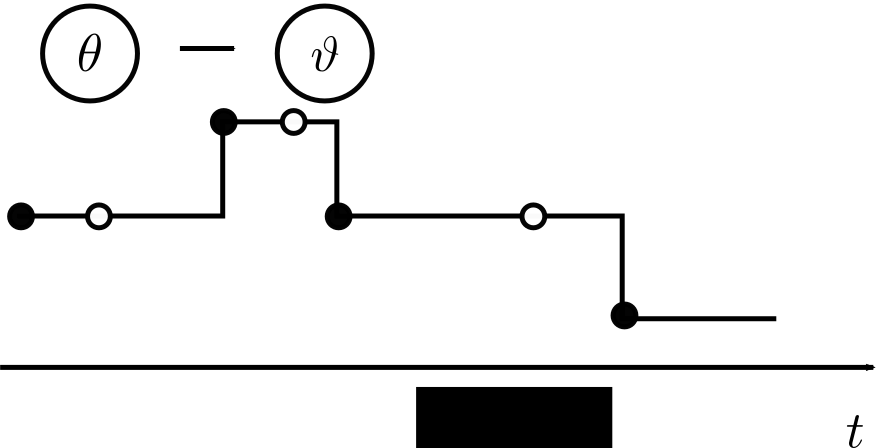
\includegraphics [width=0.90\textwidth, angle=0]{figs/plot2.pdf}
    \vspace{-0 in}
  \end{minipage}
  \begin{minipage}[hp]{0.45\linewidth}
  \centering
    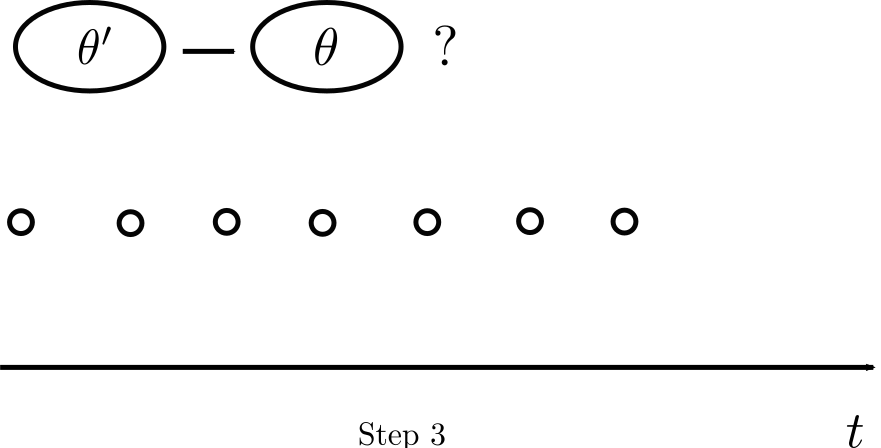
\includegraphics [width=0.90\textwidth, angle=0]{figs/plot3.pdf}
    \vspace{-0 in}
  \end{minipage}
% \begin{minipage}[hp]{0.45\linewidth}
% \centering
%   \includegraphics [width=0.70\textwidth, angle=0]{figs/plot4.pdf}
%   \vspace{-0 in}
% \end{minipage}
  \begin{minipage}[hp]{0.45\linewidth}
  \centering
    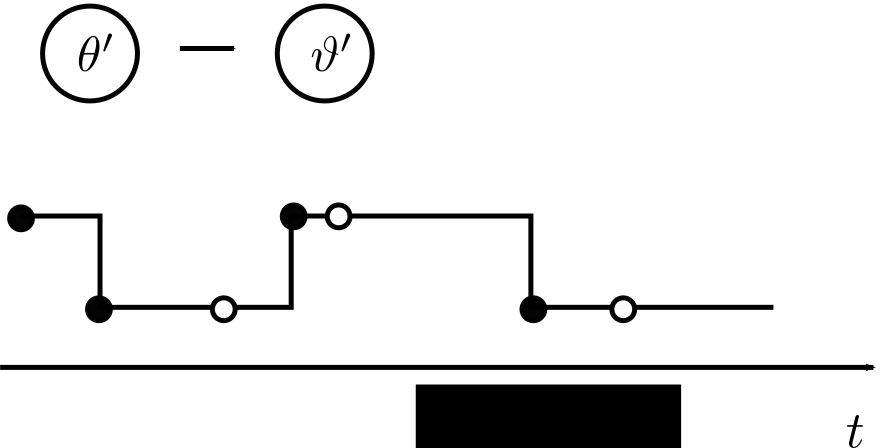
\includegraphics [width=0.90\textwidth, angle=0]{figs/plot5.pdf}
    \vspace{-0 in}
  \end{minipage}
  \begin{minipage}[hp]{0.45\linewidth}
  \centering
    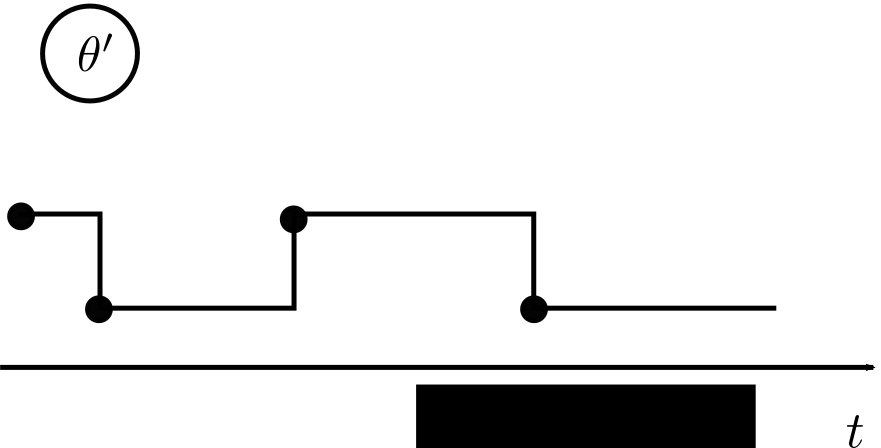
\includegraphics [width=0.90\textwidth, angle=0]{figs/plot6.pdf}
  \end{minipage}
    \caption{Proposed MH algorithm: Steps 0-3: Starting with a trajectory and parameter $\theta$, simulate an auxiliary parameter $\vartheta$, and then the thinned events
      $U$ from a rate $\Omega(\theta) + \Omega(\theta^*) - A_{S(t)}$ Poisson
      process. Step 4: Propose swapping $\theta$ and $\vartheta$. Step 5:
      Run a forward pass to accept or reject this proposal, and use the accepted
    parameter to simulate a new trajectory. Step 6: Discard $\vartheta'$ and the thinned events.} 
   \label{fig:MH_improved}
  \end{figure}
As before, the MCMC iteration begins with the pair $(S(t), \theta)$. 
Instead of simulating the Poisson events $U$, we first generate a new 
parameter $\vartheta$ from $q(\vartheta|\theta)$. Treat this as an 
auxiliary variable, so that the augmented space now is the triplet 
$(S(t), \theta,\vartheta)$. We pretend $S(t) \equiv (S,T)$ was sampled by  
uniformization, where the dominating Poisson rate $\Omega$ equals 
$(\Omega(\theta) + \Omega(\vartheta))$ instead of just $\Omega(\theta)$:
recall any choice greater than $\max_s A_s$ is valid.
Now the set of thinned events $U$ is piecewise-constant
Poisson with intensity $\Omega(\theta) + \Omega(\vartheta) - 
A_{S(t)}$. Following algorithm~\ref{alg:Unif_gibbs} or~\cite{RaoTeh13}, 
the {\em a priori} probability of the reconstructed set $W = U \cup T$, 
$P(W|\theta,\vartheta)$, is a homogeneous Poisson 
%the union of $U$ with the actual trajectory transition times $T$, 
process with rate $\Omega(\theta) + \Omega(\vartheta)$. Discard all 
MJP state information, so that the MCMC state space is $(W, \theta, \vartheta)$,
and propose swapping $\theta$ with $\vartheta$. 
Observe from
symmetry that the Poisson skeleton $W$ has the same probability both
before and after this proposal, so that unlike the previous scheme,
the ratio $P(W|\vartheta)/P(W|\theta)$ equals $1$.  This simplifies 
computation, and significantly improves mixing.
The acceptance probability 
%depends only on the probability of the observations
%under both set of parameters, %as we can use the forward-backward algorithm
%to calculate this. Our acceptance probability 
equals
$ 
  \min\left(1, \frac{P(X,\vartheta)q(\theta|\vartheta)}
   {P(X,\theta)q(\vartheta|\theta)}\right) = 
  \min\left(1, \frac{P(X|\vartheta)p(\vartheta)q(\theta|\vartheta)}
   {P(X|\theta)p(\theta)q(\vartheta|\theta)}\right).
   $
   The terms $P(X|\vartheta)$ and  $P(X|\theta)$ can be calculated by 
   running a forward pass of the forward-backward algorithm, and after
   accepting or rejecting the proposal, a new trajectory is sampled by
   completing the backward pass. Finally, the thinned events are
   discarded. Algorithm~\ref{alg:MH_improved} and 
   figure~\ref{fig:MH_improved} outline the details. 


%\subsection{Correctness of the proposed algorithm }
%\label{sec:verify2}
\begin{proposition}
  The sampler described in Algorithm~\ref{alg:MH_improved} has the posterior
  distribution $p(\theta,S(t)|X)$ as its stationary distribution.
\end{proposition}
\begin{proof}
  Suppose that at the start of the algorithm, we have a pair $(\theta,S(t))$ from
  the posterior distribution $p(\theta,S(t)|X)$. Introducing $\vartheta$
  from $q(\vartheta|\theta)$ results in a triplet whose marginal over the first
  two variables is still $p(\theta,S(t)|X)$.

  Sampling $U$ from a Poisson process with rate $\Omega(\theta) +
  \Omega(\vartheta) - A_{S(t)}(\theta)$, results in a random grid $W = T \cup U$
  that is distributed according to a rate $\Omega(\theta) + \Omega(\vartheta)$
  Poisson process (Proposition 2 in~\cite{RaoTeh13}). Discarding all state 
  information results in a triplet $(W,\theta,\vartheta)$ with probability
  proportional to $p(\theta)q(\vartheta|\theta)p(W|\theta,\vartheta)
  p(X|W,\theta,\vartheta)$.

Next we propose swapping $\theta$ and $\vartheta$. Since this
is a deterministic proposal, the MH-acceptance probability is given by
$$\alpha = 1 \wedge \frac{p(\vartheta)q(\theta|\vartheta)p(W|\vartheta,\theta)
p(X|W,\vartheta,\theta)}{p(\theta)q(\vartheta|\theta)p(W|\theta,\vartheta)
p(X|W,\theta,\vartheta)}$$
The term $p(W|\theta,\vartheta)$ is just a Poisson process with rate $\Omega(\theta)+
\Omega(\vartheta)$, so that $p(W|\theta,\vartheta) = p(W|\theta,\vartheta)$. 
$p(X|W,\theta,\vartheta)$ and $p(X|W,\vartheta,\theta)$ are obtained
after a forward pass over $W$ using discrete-time transition matrices
$B(\theta,\vartheta) = \left(I + \frac{A(\theta)}{\Omega(\theta)+\Omega(\vartheta)}\right)$ 
and $B(\vartheta,\theta) = \left(I + \frac{A(\vartheta)}{\Omega(\theta)+\Omega(\vartheta)}\right)$. 

Calling the parameters 
after the accept step $(\theta', \vartheta')$, we have that
$(\theta', \vartheta',W)$ has the same distribution as
$(\theta, \vartheta,W)$.
Finally, following Lemma 1 in~\cite{RaoTeh13}, using the matrix 
$B(\theta,\vartheta)$ to make a backward pass through $W$,
and discarding the self-transitions results in a trajectory $(S'(t)$
distributed according to $A(\theta')$. Discarding the auxiliary parameter
$\vartheta'$ results is a pair $(\theta',S'(t))$ from
the posterior.
% \begin{align*}
%  p(y, W, S, T, \theta, \theta^*) &= p(\theta) q(\theta^* | \theta) P(S,T| \theta, \theta^*) P(W| S, T, \theta, \theta^*)P(y | S, T, \theta, \theta^*)\\
%  &=p(\theta) q(\theta^* | \theta) P(S,T| \theta) P(W| S, T, \theta, \theta^*)P(y | S, T).
% \end{align*}
% The marginal distribution of $(y, S, T, \theta, \theta^*)$ and $(y, S, T, \theta)$ as follows.\\
% \begin{align*}
%  p(y, S, T, \theta, \theta^*) &= p(\theta) q(\theta^* | \theta) P(S,T| \theta, \theta^*)P(y | S, T, \theta, \theta^*)\\
%  &=P(y, S, T, \theta) q(\theta^* | \theta).
% \end{align*}
% \begin{align*}
%  p(y, S, T, \theta) &= p(\theta)P(S,T| \theta)P(y | S, T, \theta).
% \end{align*}
% So the conditional distribution over $\theta^*$ given $(y, S, T, \theta)$ is $q(\theta^* | \theta)$. And the conditional distribution over W given $(y, S, T, \theta, \theta^*)$  is $P(W | S, T, \theta, \theta^*)$, which is actually the distribution of Non Homogeneous Poisson Process with piecewise constant rate $h(\theta) + h(\theta^*) - A_{S(t)}(\theta)$.\\
% Thus the Step 1 + Step 2 is actually equivalent to sampling from the conditional distribution $P(\theta^* , W| S, T, \theta, y)$.\\
% The Step 3 + Step 4 satisfy the detailed balance condition. The reason is as follows.
% \begin{align*}
% &P((W, S, T, (\theta, \theta^*)) \rightarrow (W, S^*, T^*, (\theta^*, \theta))) P(S,T, (\theta, \theta^*) | W, y)\\
% &= (1 \wedge \frac{P((\theta^*,\theta) | W, y)}{P((\theta,\theta^*) | W, y)})P(S^*, T^* | W, (\theta^*, \theta), y)P(S, T | W, (\theta, \theta^*), y)P((\theta, \theta^*) | W, y)\\
% &= P((W, S^*, T^*, (\theta^*, \theta)) \rightarrow (W, S, T, (\theta, \theta^*))) P(S^*,T^*, (\theta^*, \theta) | W, y)
% \end{align*} 
% Therefore the stationary distribution of this MCMC sampler is $P(W, S, T, (\theta, \theta^*) | y)$. Thus the stationary distribution of $(S, T, \theta)$ is the corresponding marginal distribution $P(S, T, \theta | y)$.  
\end{proof}

\subsection{Comments}\label{sec:comments}

The uniformization scheme of~\cite{RaoTeh13} works for any underlying Poisson
process whose rate $\Omega$ is greater than $\max_i A_i$. The strict inequality
ensures that the conditional probability of sampling one or more thinned events 
$U$ is positive for every trajectory $S(t)$ (recall 
$U \sim \text{PoissonProc}(\Omega-A_{S(t)})$). Empirical results from~\cite{RaoTeh13}
suggest setting $\Omega = 2 \max_i A_i$.

Implicit in our new scheme is a uniformizing Poisson process with rate
$\Omega(\theta,\vartheta) = \Omega(\theta) + \Omega(\vartheta)$. For our 
scheme to be valid, $\Omega(\theta,\vartheta)$ must be greater than both
$\max_i A_i(\theta)$ and $\max_i A_i(\vartheta)$. The smallest and simplest such
choice is $\Omega(\theta,\vartheta) = \max A_i(\theta) + \max A_i(\vartheta)$.
For a fixed $\theta$, this reduces to $\Omega = 2\max A_i$, providing
an intuitive motivation for the approach in~\cite{RaoTeh13}.
Larger alternatives include 
$\Omega(\theta,\vartheta) = \kappa(\max A_i(\theta) + \max A_i(\vartheta))$
for $\kappa > 1$.  These result in more thinned events, and therefore more 
computation, with the benefit of faster MCMC mixing. We study the effect of 
$\kappa$ in our experiments.

It is also possible to have non-additive settings for $\Omega(\theta,\vartheta)$.
A simple option is to set it equal to 
$\kappa \max( \max_i A_i(\theta), \max A_i(\vartheta))$ for some choice of $\kappa
> 1$. We investigate this option as well.

Our proposed algorithm is related to work on MCMC inference for doubly-intractable distributions.
Algorithm like~\cite{Moller2006,murray2006,Andrieu09} all attempt to evaluate an intractable
likelihood under a proposed parameter $\theta^*$ by introducing auxiliary variables, however there
the auxiliary variable is sampled independently under the proposed parameters. For MJP, this would
involve proposing a new parameter $\theta^*$, generating a new uniformizing grid $U^*$, and then
accepting or rejecting. This can complicate computations (with two sets of time points), and also
reduce acceptance rates if
 the new parameter $\theta^*$ is incompatible with the old grid $U$ or
vice versa. While~\cite{murray2006} suggest annealing schemes to try to address this issue, we exploit
the structure of the Poisson process and provide a cleaner solution: generate a single set of
auxiliary variables that depends symmetrically on both the new and old parameters. It is interesting
to see whether a similar idea can be used in other applications as well.


\section{Experiments}\label{sec:expts}~
In the following, we evaluate Python implementations of our two proposed
algorithms, the \naive\ MH algorithm (algorithm~\ref{alg:MH_naive}, which we
plot in yellow) and its symmetrized improvement (algorithm~\ref{alg:MH_improved}, 
which we call symmetrized MH and plot in red). We compare different variants of 
these algorithms, corresponding to different uniformizing Poisson rates 
(i.e.\ different choices of $\kappa$, see section~\ref{sec:comments}). For 
\naive\ MH, %~\ref{alg:MH_naive}, 
we set $\Omega(\theta) = \kappa \max_s A_s(\theta) $ with $\kappa$  equal to 
$1.5, 2$ and $3$, represented in our plots with circles, triangles and square
symbols. For symmetrized MH, %algorithm~\ref{alg:MH_improved}, 
where the uniformizing rate depends 
on both the current and proposed parameter, we consider two settings
 $\Omega(\theta, \theta^*) = \kappa (\max A(\theta) + \max A(\theta^*))$ 
 ($\kappa = 1$ and $1.5$, plotted with circles and triangles), and 
$\Omega(\theta, \theta^*) = \kappa \max(\max A(\theta), \max A(\theta^*))$
($\kappa=1.5$, plotted with squares).  We compare these
algorithms against two baselines: Gibbs sampling (algorithm~\ref{alg:MJP_gibbs},
plotted in blue), and particle MCMC~\cite{Andrieu10}, plotted in black. Gibbs
sampling involves a uniformization step to update the MJP trajectory, and for this
we used three settings, $\kappa=1.5,2,3$, plotted with circles, squares and
triangles.  Unless specified, our results were
obtained from $100$ independent MCMC runs, each consisting of $10000$ iterations.
We found particle MCMC to be more computationally intensive, and limited each 
run to $3000$ iterations, the number of particles being $5, 10$ and $20$ 
(plotted with circles, trianges and squares). 

% We also considered exploiting gradient information of the target distribution to 
% apply Hamiltonian Monte Carlo (HMC)~\cite{Neal2010}. In particular, the forward 
% pass of FFBS allows us to also calculate the gradient of the log-probability with
% respect to the MJP parameters. We can exploit this information for more directed
% explorations of parameter space than a random-walk algorithm. Of course, this 
% comes at a higher computational cost. We evaluate HMC with the number of leapfrog
% steps taking values in $1, 3, 5$ or $10$, and the leapfrog stepsize taking values 
% in $0.02, 0.05$ and $0.1$. 

For each run of each MCMC algorithm, we calculated the effective sample size 
(ESS) of the posterior samples of the MJP parameters using the R package 
\texttt{rcoda}~\cite{Rcoda2006}. This estimates the number of independent 
samples returned by the MCMC algorithm, and dividing this by the runtime of a 
simulation gives the ESS per unit time. We used this measure to compare 
different samplers and different parameter settings.

% \begin{algorithm}[!ht]
%    \caption{Generic Gibbs sampling for MJPs for Gamma priors}
%    \label{alg:Generic Gibbs}
% \begin{algorithmic}
%    \State {\bfseries Input:} observations $y_{[t_0, t_{k+1})}$
%    \State Initialize, $i = 0$
%    \\ (a) Set $\alpha(0), \beta(0)$ arbitrarily and set current trajectory $[S,T](0)$ arbitrarily.\\
%     (b) Uniformize $[S,T](0)$, to get virtual jumps $U$.
%    \Repeat
%    \For{$i=1$ {\bfseries to} $N$}
%     \State (a) Sample $U(i) \sim P( U | \beta(i - 1), \alpha(i - 1), S(i - 1), T(i - 1), y)$.\\	
%     \State (b) Use FFBS algorithm to  sample states given all the jump times(both true jumps and virtual jumps).
% (i.e. $V(i) \sim P(V |  \beta(i - 1), \alpha(i - 1), W(i ), y).$) Then delete all the virtual jumps to get $S(i), T(i) .$\\
%     \State (c) Propose $\beta^* \sim q(.| \beta(i -1))$.\\
%       Set $\beta(i) = \beta^*$, with probability $P_{acc} = 1 \wedge \frac{P(\beta^* |S(i), T(i))}{P(\beta(i - 1) |S(i), T(i))} \frac{q(\beta(i - 1)|\beta^*)}{q(\beta^*|\beta(i - 1))}$;\\Otherwise set $\beta(i) = \beta(i-1)$.\\	  
%     \State (d) Sample $\alpha(i) \sim P(. | \beta(i), S(i), T(i), y)$.\\ It is a $Gamma(\mu + N, \lambda + \sum_{0}^NF_{S_i}(\beta)(t_{i + 1} - t_i))$ distribution actually.\\
%     \EndFor
%     \Until{$ i = N$ }
%  \end{algorithmic}
%  \end{algorithm}

\subsection{A simple synthetic MJP}
  \begin{figure}[H]
  \centering
  \begin{minipage}[!hp]{0.45\linewidth}
  \centering
    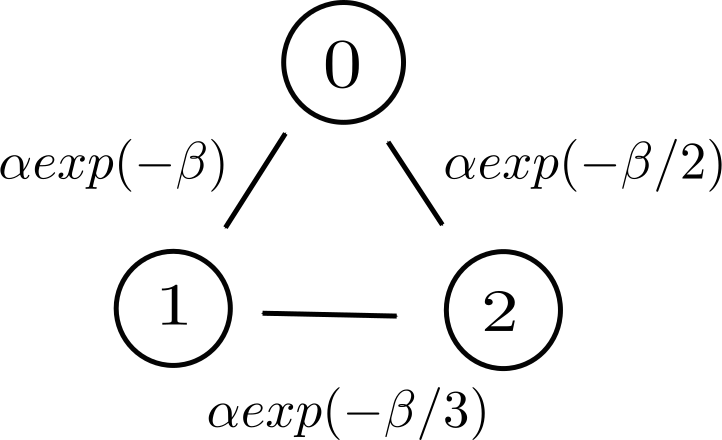
\includegraphics [width=0.70\textwidth, angle=0]{figs/exp_model.pdf}
      \end{minipage}
    \caption{A 3-state MJP with exponentially decaying rates}
    \label{fig:exp_model}
  \end{figure}

% \noindent Assume: $S = [S_0,S_1, ...,S_N] \;, T = [t_0(t_{start}), t_1,...,t_N, t_{N+1}(t_{end})]$, and y as observations.\\
% We consider a specific structure of rate matrix $A$. $A_{ij} = \alpha f_{ij}(\beta), \; i \neq j$. $A_{ii} = -\sum_{j \neq i} A_{ij}$. $0 \leq f_{ij} \leq 1$. Denote $F_i(\beta) = \sum_{j \neq i} f_{ij}(\beta)$.\\
% \begin{align*}
% P(s_0, S, T | \alpha, \beta) &= \pi_0(s_0)\prod_{i = 1}^N A_{S_{i - 1}S_i} \exp(- \int_{t_{start}}^{t_{end}} |A_{S(t)}| dt)\\
% &= \pi_0(s_0) \alpha^N \prod_{i = 1}^N f_{S_{i - 1}S_i} \exp(-\alpha  \sum_{i = 0}^{N} F_{S_i}(\beta)(t_{i + 1} - t_i))\\
% \end{align*} 
\noindent Consider an MJP with two parameters $\alpha$ and $\beta$, 
transitions between states $i$ and $j$ having rate $\alpha \exp(-\beta/(i+j))$.
We consider three settings: $3$ states (figure~\ref{fig:exp_model}),
$5$ states, and $10$ states.
We place Gamma$(\alpha_0,\alpha_1)$, and Gamma$(\beta_0, \beta_1)$ priors on 
the parameters $\alpha$ and $\beta$, with $(\alpha_0,\alpha_1,\beta_0,\beta_1)$ 
having values $(3,2,5,2)$ respectively. For each run, we draw random parameters 
from the prior to construct a transition matrix $A$, and placing a uniform 
distribution over states at time $0$, simulate an MJP trajectory.
We simulate observations uniformly at integer values on the time interval 
$[0, 20]$. Each observation is Gaussian distributed with mean equal to the state
at that time, and variance equal to $1$.  For the Metropolis-Hastings proposal, 
we used a lognormal distribution centered at the current parameter value, with 
a user-specified variance.
%\vinayak{We studied our MH sampler, for three setting of $k$}.  
% %\begin{align*}
% %P(\alpha, \beta | s_0, S, T ) \propto \alpha^N \prod_{i = 1}^N f_{S_{i - 1}S_i} \exp(-\alpha  \sum_{i = 0}^{N} F_{S_i}(\beta)(t_{i + 1} - t_i)) p_1(\alpha)p_2(\beta)\\
% %\end{align*}
% %If we assume the priors of $\alpha$, $\beta$ are $Gamma(\mu, \lambda)$, $Gamma(\omega, \theta)$, then the posterior will have a simper form as follows. 
% \begin{align*}
% P(\alpha, \beta | s_0, S, T ) = C \alpha^{\mu + N - 1}\exp(-\alpha (\lambda + \sum_{i = 0}^{N} F_{S_i}(\beta)(t_{i + 1} - t_i))) \prod_{i = 1}^N f_{S_{i - 1}S_i}  \beta ^{\omega - 1} \exp(-\theta \beta)\\
% \end{align*}
% We notice that given $\beta,\; S,\; T$, $\alpha$ is distributed as a $Gamma$ distribution.\\
% $\alpha | \beta, S, T, y  = \alpha | \beta, S, T \sim Gamma(\mu + N, \lambda + \sum_{0}^NF_{S_i}(\beta)(t_{i + 1} - t_i))$.\\
% There is no conjugate distribution to sample $\beta \sim P(\beta| s_0, S, T)$. We will have to use Metropolis Hasting within Gibbs to sample $\beta$. The target distribution is the following one.
% $$ P(\beta | S, T) = C \frac{\prod_{i = 1}^N f_{S_{i -1}S_i}(\beta)\beta^{\omega - 1} \exp(-\theta \beta)}{(\lambda + \sum_{i = 0}^{N} F_{S_i}(\beta)(t_{i + 1} - t_i))^{\mu + N}}.$$
% Such doubling might slow the mixing of the Markov chain. We can apply our Metropolis Hasting algorithm on this model.

\noindent \textbf{Results:}
  \begin{figure}%[b]
  \centering
  \begin{minipage}[!hp]{0.95\linewidth}
  \centering
    \includegraphics [width=0.45\textwidth, angle=0]{figs/exp_3_alpha.pdf}
    \includegraphics [width=0.45\textwidth, angle=0]{figs/exp_3_beta.pdf}
  \vspace{-1in}
  \end{minipage}
  \begin{minipage}[!hp]{0.95\linewidth}
  \centering
    \includegraphics [width=0.45\textwidth, angle=0]{figs/exp_10_alpha.pdf}
    \vspace{-0 in}
    \includegraphics [width=0.42\textwidth, angle=0]{figs/exp_10_beta.pdf}
    \vspace{-0 in}
  \end{minipage}
    \caption{ESS/sec for the synthetic  model, the top row being dimension 3, and the bottom,
      dimension 10. The left column is for $\alpha$, and the 
    right is for $\beta$. Red, yellow, blue and black curves are the symmetrized MH,
  \naive\ MH, Gibbs and particle MCMC algorithm. Different symbols correspond
to different settings of the algorithms, see section~\ref{sec:expts}}
     \label{fig:ESS_EXP_D10}
  \end{figure}
  Figure~\ref{fig:ESS_EXP_D10} plots the ESS per unit time for the parameters 
  $\alpha$ (left) and $\beta$ (right) for the
  case of $3$ states (top row) and $10$ states (bottom row) as we vary the scale-parameter $\sigma^2$ of the
  log-normal proposal distribution. We include results for $5$ states in the 
  supplementary material, the conclusions are the same. 
  %as we change the variance of the
  %proposal kernel, for different methods and different scaling parameters.
  %($\kappa =
%1.5, 2, 3$) and dimensions($p = 3, 5, 10$).
%, where   $k = 1.5$,  $\Omega(\theta, \theta^*) = k \max(\max A(\theta), \max A(\theta^*))$. 
%For particle MCMC, the number of particles can be $5, 10 , 20$. 
%  Blue lines are the Gibbs sampler, orange lines are \naive\ MH, red lines 
%are the symmetrized MH and black lines are particle MCMC. 
%For methods involving standard uniformization (Gibbs and \naive\ MH), dots 
%correspond to $\kappa = 1$, triangles correspond to $\kappa = 2$, and squares 
%correspond to $\kappa = 1.5$. For our symmetrized MH algorithm, circles,
%triangles and squares correspond to $\Omega = (\Omega_{old} + \Omega_{new}),
%2(\Omega_{old} + \Omega_{new})$ and $1.5 \max(\Omega_{old}, \Omega_{new})$
%respectively, where $\Omega_{new}$ and $\Omega_{old}$ equal $\max_i A_i$ under 
%the proposed and current parameters.
%  For particle MCMC, the dot-dashed lines correspond to 
%  $5$ particles,  the dashed lines correspond to $10$ particles, and the solid 
%  lines correspond to $20$ particles.
We see that our symmetrized MH algorithm is significantly more efficient 
than the baselines over a wide range of choices of $\sigma^2$, 
(including the natural choice of $1$).
Among the three setting of our algorithm, the simple additive setting
 (circles) does best, though it is not significantly better than the additive
 setting with a multiplicative factor of $2$ (triangles). The max-of-max setting
 (squares) does worse than both additive choices but still better than the
 other algorithms.  Among the baselines, simple Gibbs sampling 
does better than \naive\ Metropolis-Hastings, suggesting that the dependency of 
the Poisson grid on the MJP parameters does indeed significantly slow 
down mixing. Particle MCMC has the worst performance for this task. The
results in figure~\ref{fig:ESS_EXP_D10} for the 10-dimensional state space
show that for the parameter $\alpha$, the improvement that our proposed
sampler affords is even more dramatic. For the parameter $\beta$ however,
it's performance is comparable to Gibbs, although it's not possible to
claim one is uniformly superior to the other.

  \begin{figure}%[b]    
  \centering
  \begin{minipage}[hp]{0.24\linewidth}
  \centering
    \includegraphics [width=0.99\textwidth, angle=0]{figs/ESS_vs_t_alpha_fixobservation.pdf}
    \end{minipage}
  \begin{minipage}[hp]{0.24\linewidth}
  \centering
    \includegraphics [width=0.99\textwidth, angle=0]{figs/ESS_vs_t_beta_fixobservation.pdf}
%    \vspace{-0.3in}
  \end{minipage}
    %\label{fig:TSS_fix}
  \begin{minipage}[hp]{0.24\linewidth}
  \centering
    \includegraphics [width=0.99\textwidth, angle=0]{figs/ESS_vs_t_alpha.pdf}
      \end{minipage}
  \begin{minipage}[hp]{0.24\linewidth}
  \centering
    \includegraphics [width=0.99\textwidth, angle=0]{figs/ESS_vs_t_beta.pdf}
  \end{minipage}
    \vspace{-0.3in}
%    \caption{Time Interval vs. ESS / sec}
    \caption{Time Interval vs. ESS/sec. In the left two plots, the number of 
    observations is fixed, in the right two, this grows linearly with the
  interval length. Red, yellow and blue curves are the symmetrized MH,
  \naive\ MH and Gibbs algorithm.}
     \label{fig:TSS}
  \end{figure}
%We generate different observations on different time intervals.
%Our observation process was a Gaussian distribution with mean equal to the 
%current state and variance equal to $1$. 
In figure~\ref{fig:TSS}, we plot ESS per unit time as the observation 
interval $\cT$ increases. We consider the three-state MJP, and as before there 
are $19$ observations uniformly located over a time interval $(0,\cT)$. We 
consider four settings, with $\cT$ equal to $10, 20, 50, 100$. For each, we 
compare our symmetrized MH sampler (with $\kappa$ set to $1$) with the Gibbs 
sampler (with $\kappa$ set to $2$). While the performance of the Gibbs sampler 
is comparable with our symmetrized algorithm for the smallest value of 
$\cT$, its performance is considerably worse for longer time-intervals. This is 
because of the conditional nature of the updates of the Gibbs sampler, where MJP
trajectories are sampled as intermediate objects to facilitate updating the
parameters. Longer time intervals will then result in stronger coupling between 
MJP path and parameters, slowing down mixing. This effect disappears if we 
integrate out the MJP trajectory. This experiment demonstrates that it
is not sufficient just to integrate out the state values of the trajectory, 
instead, we also have to get around the effect of the
trajectory transition times. Our symmetrized MH-algorithm allows us to do
this. 
%as a by-product, it also involves calculating a simpler 
%MH acceptance probability.


In figure~\ref{fig:TSS}, we plot results from a similar experiment. Now,
instead of keeping the number of measurements fixed as we increase the 
observation interval, we keep the observation rate fixed at one observation 
every unit interval of time, so that longer observation intervals have larger 
number of observations. The results are similar to the previous case: Gibbs 
sampling performs well for small observation intervals, with performance 
degrading sharply for larger observation intervals. These two experiments 
illustrate the usefulness of our idea of integrating out the MJP path while 
carrying out parameter inference.

  \subsection{The Jukes and Cantor (JC69) model}~
  \begin{figure}%[H]
  \centering
  \begin{minipage}[!hp]{0.48\linewidth}
  \centering
    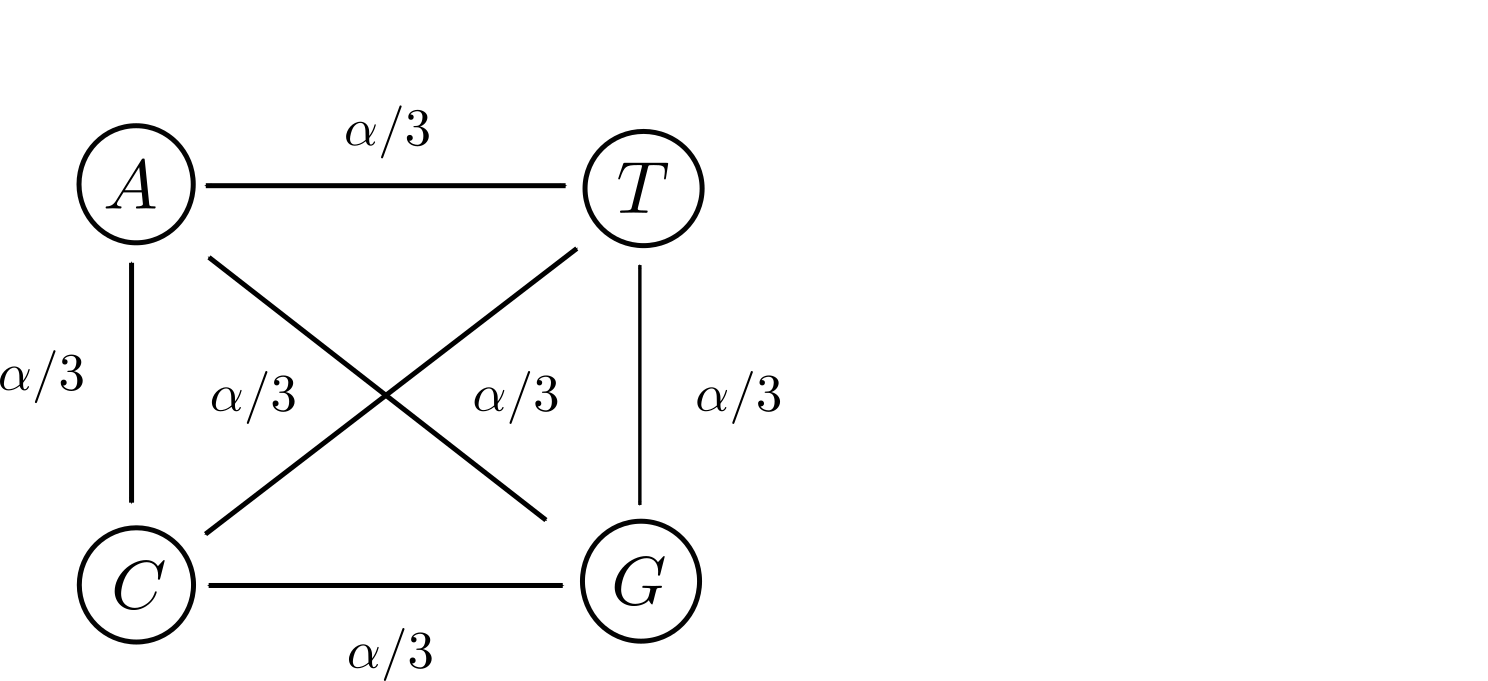
\includegraphics [width=1.07\textwidth, angle=0]{figs/jc_model.pdf}
    \caption{The Jukes and Cantor (JC69)$\qquad$  model}
	\label{jc_model}
  \end{minipage}
  \begin{minipage}[!hp]{0.46\linewidth}
  \centering
    \includegraphics [width=0.9\textwidth, angle=0]{figs/jc.pdf}
    \vspace{-0.6in}
    \caption{ESS/sec for the JC69 Model. Red, yellow and blue curves are the 
      symmetrized MH, \naive\ MH and Gibbs algorithm. }
     \label{fig:ESS_JC}
  \end{minipage}
  \end{figure}
  The Jukes and Cantor (JC69) model is a popular model of DNA nucleotide
  substitution.  We write its state space as $\{0, 1, 2, 3\}$, representing the 
  four nucleotides $\{A, T, C, G\}$.  The model has a single parameter $\alpha$, 
  representing the rate at which the system transitions between any pair of 
  states. Thus, the rate matrix $A$ is given by 
  %Assume: $S = [S_0,S_1, ...,S_N] \;, T = [t_0(t_{start}), t_1,...,t_N, t_{N+1}(t_{end})]$, and y as observations.\\
$A_i = -A_{i,i} = 3\alpha, A_{i, j} = \alpha,i \neq j.$
We place a Gamma$(3,2)$ prior on the parameter $\alpha$.
Figure~\ref{fig:ESS_JC}(right) compares different samplers: we see that the
symmetrized MH samplers comprehensively outperforms all others.
Part of the reason why the difference is so dramatic here is because the
transition matrix is no longer sparse in this example, implying a stronger
coupling between MJP path and parameter $\alpha$. We point out that for Gibbs
sampling, the conditional parameter update is conjugate, and there is no
proposal distribution involved (hence it's performance remains fixed along
the x-axis). Particle MCMC performs worse
than all the algorithms, and we do not include it in our plots.

In figure~\ref{fig:jc_model_vs_t}, we plot the ESS per unit time for the
different samplers as we increase the observation interval. In the left plot,
we keep the number of observations fixed, in the right, these increase with
the observation interval. Once again we see that our proposed algorithm
1) performs best over all interval lengths, and 2) suffers a performance
degradation with interval length that is much milder than the other algorithms.
%$$p(\alpha) = \frac{\lambda^\mu}{\Gamma(\mu)}\alpha^{\mu -1}e^{-\lambda \alpha} $$.
%Then we can get the posterior distribution $$f(\alpha | s_0,S,T)$$ as follows.
%$$ f(\alpha| s_0,S,T) \propto \exp(-(\lambda + 3(t_{end} - t_{start}))\alpha) \alpha^{\mu + N -1} .$$
%$\alpha | s_0,S,T$ is following $Gamma(\mu+ N,\lambda + 3(t_{end} - t_{start}))$\\
  \begin{figure}%[H]
  \centering
  \begin{minipage}[!hp]{0.45\linewidth}
  \centering
    \includegraphics [width=0.97\textwidth, angle=0]{figs/ESS_vs_t_alpha_JC.pdf}
  \end{minipage}
  \begin{minipage}[!hp]{0.45\linewidth}
  \centering
    \includegraphics [width=0.97\textwidth, angle=0]{figs/ESS_vs_t_alpha_fixobservation_JC.pdf}
  \end{minipage}
	\label{fig:jc_model_vs_t}
    \caption{Time Interval vs. ESS/sec. In the left plot, the number of 
    observations is fixed, in the right, this grows linearly with the
  interval length. Red, yellow and blue curves are the symmetrized MH,
  \naive\ MH and Gibbs algorithm. }
  \end{figure}


\subsection{An immigration model with finite capacity}\label{sec:immig}~
Finally, we consider an M/M/N/N queue. This is a stochastic 
process whose state space is the set $\{0, 1, 2, 3, \cdots, N - 1\}$ with 
elements giving the number of customers/jobs/individuals in a system/population. 
Arrivals follow a rate-$\alpha$ Poisson process, moving the process from state 
$i$ to $i+1$ for $i<N$. The system has a capacity of $N$, so any arrivals when 
the current state is $N$ are discarded.  Service times or deaths are 
exponentially distributed, with a rate that is now state-dependent:
the system moves from $i$ to $i - 1$ with rate $i\beta$. 
%There are $N$ servers, which serve from the front of the queue. 
%If there are less than $N$ jobs, some of the servers will be idle. 
%Only $N$ customers can queue at any one time. 
%Any further arrivals to the queue are considered ''lost''. 

% \begin{figure}
% \centering
% \begin{minipage}[hp]{0.6\linewidth}%0.45
% \centering
%   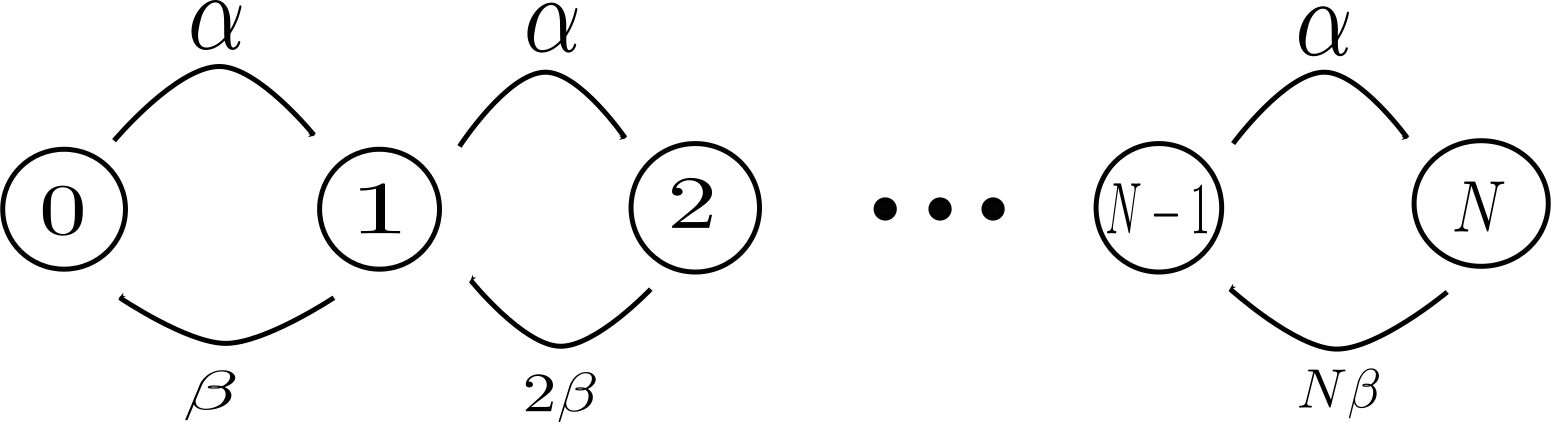
\includegraphics [width=1\textwidth, angle=0]{figs/queue_model.pdf}%0.70
%     \end{minipage}
%   \caption{queuing model}
%   \label{q_model}
% \end{figure}
  \begin{figure}%[b]
  \centering
  \begin{minipage}[hp]{0.9\linewidth}
  \centering
    \includegraphics [width=0.45\textwidth, angle=0]{figs/q_3_alpha.pdf}
    \hspace{.2in}
    \includegraphics [width=0.45\textwidth, angle=0]{figs/q_3_beta.pdf}
    \vspace{-1.0 in}
  \end{minipage}
  \begin{minipage}[!hp]{0.9\linewidth}
  \centering
    \includegraphics [width=0.45\textwidth, angle=0]{figs/q_10_alpha.pdf}
    \hspace{.2in}
    \includegraphics [width=0.45\textwidth, angle=0]{figs/q_10_beta.pdf}
    \vspace{-0.5 in}
  \end{minipage}
    \caption{ESS/sec for the immigration model, the top row being dimension 3, and the bottom,
      dimension 10. The left column is for $\alpha$, and the 
    right is for $\beta$. Red, yellow, blue and black curves are the symmetrized MH,
  \naive\ MH, Gibbs sampling and particle MCMC.}
     \label{fig:ESS_Q_D10}
  \end{figure}
We follow the same setup as the first experiment:
for $(\alpha_0,\alpha_1,\beta_0,\beta_1)$ equal to $(3,2,5,2)$,
we place Gamma$(\alpha_0,\alpha_1)$, and Gamma$(\beta_0, \beta_1)$ priors on 
$\alpha$, $\beta$. These prior distributions are used to sample transition 
matrices $A$, which, along with a uniform distribution over initial states,
are used to generate MJP trajectories. We observe these at integer-valued
times according to a Gaussian observation process.
We consider three settings: $3, 5$ and $10$ states, with results from $5$ 
steps included in the supplementary material. 

  %\subsection{Experiments}
  Figure~\ref{fig:ESS_Q_D10} plots the ESS 
  per unit time for the parameters $\alpha$ (left) and $\beta$ (right) as we 
  change the variance of the proposal kernel, for different settings of
  different algorithms. The top row shows results for a state-space
  of dimension $3$, and the bottom row, results for a dimension
  $10$ (we include the case of dimension $5$ in the supplementary material).
  %Colors and types are the same as the previous experiment.
  Again, our symmetrized  MH algorithm does best for dimensions
  $3$ and $5$, although now Gibbs sampling performs well for dimensionality $10$.
  This is partly because for the problem, the Gibbs conditionals over $\alpha$
  and $\beta$ and conjugate, and have a very simple Gamma distribution
  (this is also why the Gibbs sampler curves are straight lines: there is no
  proposal distribution involved here).
% Figure~\ref{fig:hist} shows posterior distributions for 
% $P(\theta | X)$(red), $P(\theta | S, T, X)$(green), $P(\theta | W, X)$(blue). 
% We run $10000$ iterations. The first $5000$ are treated as burn in period. 
% We fix $V_{5000}, W_{5000}$ and then sample $\theta$ from 
% $P(\theta | V_{5000}, W_{5000}, X)$ and sample $\theta$ from 
% $P(\theta | W_{5000}, X)$. We keep updating $S$ and $T$ for sampling from 
% $P(\theta | X)$. We sample another $5000$ $\theta$s to draw the histograms. 
% We can find that $P(\theta | S, T, X)$ and $P(\theta | W, X)$ are both very 
% concentrated which implies the coupling.
% \begin{figure}%[b]
% \begin{minipage}[hp]{0.45\linewidth}
% \centering
%   \includegraphics [width=0.90\textwidth, angle=0]{figs/dist_alpha.pdf}
%   \vspace{-0 in}
% \end{minipage}
% \begin{minipage}[!hp]{0.45\linewidth}
% \centering
%   \includegraphics [width=0.90\textwidth, angle=0]{figs/dist_beta.pdf}
%   \vspace{-0 in}
% \end{minipage}
%   \caption{density.The left is for $\alpha$, and the right is for $\beta$.}
%    \label{fig:dist}
% \end{figure}
\subsubsection{A time-inhomogeneous immigration model}~
Here we extend the previous model to incorporate a known time-inhomogeneity. 
The arrival and death rates are no longer constant, and are instead given by
 %$$A_i(t) =: A_{i,i}(t) = -(\alpha + i\beta)w(t), \; \; i =0,1,...,N$$ 
$A_{i, i+1}(t) = \alpha w(t) \ (i =0,1,\cdots,N-1)$ respectively.
While it is not difficult to work with sophisticated choices of $w(t)$,
here we limit ourselves to a simple piecewise-constant choice of $w(t)$ 
given by $w(t) = \left\lfloor \frac{t}{5} \right\rfloor$. Even such a simple
change in the original model can dramatically affect the performance
of the Gibbs sampler.
% $w(t) = w_i, \; t \in [\l_i, l_{i + 1}), i = 1,2,3,..., K$.
%\noindent Assume: $S = [S_0,S_1, ...,S_N] \;, T = [t_0(t_{start}), t_1,...,t_N, 
%t_{N+1}(t_{end})]$, and y as observations.\\
%Now, let's consider a immigration model as follows. State space is 
% $\{0, 1, 2, ..., N - 1\}$, representing the total population. 
% We already know the conditional density(given $\alpha,\; \beta$) of a MJP trajectory $(s_0, S, T)$ in time interval $[t_{start}, t_{end}]$, with $S=(s_1, s_2,..., s_k)$, $T=(t_1, t_2,..., t_k)$. 
% $$f(s_0,S,T| \alpha, \beta) = \prod_{i=0}^{k-1} A_{s_i, s_{i+1}}(t_i) \exp(\sum_{i=0}^{k} A_{s_i}(t_i)(t_{i+1} - t_{i})), $$
% where $t_0 = t_{start}$, $t_{k+1} = t_{end}.$\\
% Let's denote some notations here.\\
% $$U(s_0, S, T):= \sum_{i=0}^{k-1} \mathbb{I}_{\{s_{i+1} - s_i = 1\}}.$$
% $$D(s_0, S, T):= \sum_{i=0}^{k-1} \mathbb{I}_{\{s_{i+1} - s_i = -1\}}.$$
% Call them U and D for short.
% Let's denote the total time when the trajectory state stays at state i as $\tau_i$, i.e. $\tau_i = \sum_{j=0}^{k} (t_{j+1} -t_j)\mathbb{I}_{\{s_j = i\}}$, then $\sum_{i=0}^k (t_{i+1} - t_i)s_i = \sum_{i=0}^N \tau_ii.$\\

% $$f(s_0,S,T| \alpha, \beta) \propto \exp(\sum_{r = 0}^{K}-w_r\alpha(l_{r + 1} - l_{r}- \tau_N^r) )\alpha^U \cdot  \exp(-\int_{t_s}^{t_{e}}(S(t)w(t)\beta)  \beta^D$$\\
% If we assume the prior of $\alpha$, and $\beta$ are $Gamma(\mu,\lambda)$, $Gamma(\omega, \theta)$, which are independent with each other. \\
% $$p(\alpha) = \frac{\lambda^\mu}{\Gamma(\mu)}\alpha^{\mu -1}e^{-\lambda \alpha}. $$
% $$p(\beta) = \frac{\theta^\omega}{\Gamma(\omega)}\beta^{\omega -1}e^{-\theta \beta}. $$
% Then we can get the posterior distribution $$f(\alpha, \beta | s_0,S,T)$$ as follows.
% $$ f(\alpha, \beta | s_0,S,T) \propto \exp(-(\lambda +\sum_{r = 0}^{K}w_r\alpha(l_{r + 1} - l_{r}- \tau_N^r))\alpha) \alpha^{\mu + U -1} \cdot \exp(-(\int_{t_{s}}^{t_{e}}(S(t)w(t) + \theta)\beta) \beta^{\omega+ D -1}.$$
% It means that the posterior distributions of $\alpha$, $\beta$ are still independent. \\
% $\alpha | s_0,S,T$ is following $Gamma(\mu+ U,\lambda +\sum_{r = 0}^{K}w_r\alpha(l_{r + 1} - l_{r}- \tau_N^r)  )$\\
% $\beta | s_0,S,T$ is following $Gamma(\omega+ D,\int_{t_s}^{t_{e}}(S(t)w(t) + \theta)$.\\
% Such immigration models have perfectly conjugate posterior distributions when we assign $\gamma$ priors to $\alpha$ and $\beta$. We apply our Metropolis Hasting algorithms on such models to compare the performance with the performance of Gibbs Sampling algorithm.

%\subsection{Experiments}

 The top row of figure~\ref{fig:ESS_pc_10} plots the ESS per unit time for the 
 parameters $\alpha$ (left) and $\beta$ (right) for the immigration model with 
 capacity $3$.  Now, the symmetrized MH algorithm is significantly 
 more efficient, comfortably outperforming all samplers (including the Gibbs 
 sampler) over a wide range of settings. %The Gibbs sampler slightly outperforms
 %the simple MH sampler, while particle MCMC is significantly worse (we have
% not included it).  
 Figure~\ref{fig:ESS_pc_10} shows performance for dimension
 $10$, once again the symmetrized MH-algorithm performans best over a 
 range of settings of the proposal variance. We note that increasing the
 dimensionality of the state space results in a more concentrated posterior,
 shifting the optimal setting of the proposal variance to smaller values.
  \begin{figure}%[b]
  \centering
  \begin{minipage}[!hp]{0.9\linewidth}
  \centering
    \includegraphics [width=0.42\textwidth, angle=0]{figs/pc_3_alpha.pdf}
    \hspace{.2 in}
    \includegraphics [width=0.42\textwidth, angle=0]{figs/pc_3_beta.pdf}
    \vspace{-.81 in}
  \end{minipage}
  \begin{minipage}[!hp]{0.9\linewidth}
  \centering
    \includegraphics [width=0.420\textwidth, angle=0]{figs/pc_10_alpha.pdf}
    \hspace{.2 in}
    \includegraphics [width=0.420\textwidth, angle=0]{figs/pc_10_beta.pdf}
    \vspace{-.5in}
  \end{minipage}
    \caption{ESS/sec for the time-inhomogeneous immigration model, the top row 
      being dimension 3, and the bottom,
      dimension 10. The left column is for $\alpha$, and the 
    right is for $\beta$. Red, yellow and blue curves are the symmetrized MH,
  \naive\ MH, and Gibbs algorithm.}
     \label{fig:ESS_pc_10}
  \end{figure}


%\input{ergodicity_mar20.tex}
\section{Geometrical ergodicity}
\begin{assumption}
$\exists$ $k_2 > k_1 > 1$ and $\epsilon_1, \epsilon_2 > 0$, s.t. $k_2 ( \{ \max_s|A_{ss}(\theta)| +  \max_s|A_{ss}(\nu)| ) + \epsilon_2 \geq \Omega(\theta, \nu)$ and $\Omega(\theta, \nu) \geq k_1 \max \{ \max_s|A_{ss}(\theta)|, \max_s|A_{ss}(\nu)| \} + \epsilon_1.$ 
\end{assumption}

\begin{assumption}
Given the proposal density $q(\mu | \theta)$, $\exists \eta_0 \in (0, 1)$ s.t. $$ \int_\Theta \max_s|A_{ss}(\nu)| q(\nu | \theta)d\nu \leq \eta_0 \max_s|A_{ss}(\theta)|.$$
\end{assumption}

\begin{assumption}
$\exists$ $ \xi_1 > \eta_1 > 0$ s.t. $\prod P(x_o | s_o, \theta) \in (\eta_1, \xi_1)$.
\end{assumption}



\begin{assumption}
For the ideal sampler with the proposal density $q(\nu| \theta)$ and the acceptance rate $\alpha_i(\theta, \nu) = 1 \wedge \frac{P(X | \nu)q(\theta| \nu)p_0(\nu)}{P(X | \nu)q(\nu| \theta)p_0(\theta)}$, $\exists$ a probability measure $\phi$, a constant $\kappa_1 > 0$ and a set $C \subseteq \Theta$, s.t. $q(\nu | \theta) \alpha_i(\theta, \nu) \geq \kappa_1 \phi(\nu)$ for $\theta \in C$. 
\end{assumption}

\begin{assumption}
For the above $C \subseteq \Theta$, $\exists$ $\bar{\Omega} > 0$ s.t. $\Omega(\theta, \nu)  \leq \bar{\Omega}$ for $\forall (\theta, \nu) \in C \times C$.
\end{assumption}

\begin{theorem}
Under the above assumptions, for $\forall h > 0$, the set $\{ (W, \theta, \theta^*) | |W| \leq h, \theta \in C \}$ is a small set.
\end{theorem}
\begin{proof}
\begin{align*}
P(W', \nu, \theta | W, \theta, \theta^*) &\geq q(\nu | \theta)\alpha(\theta, \nu, W') \int_T \sum_S P(S,T | W, \theta, \theta^*, X) P(W'| S, T, \theta, \nu)dT  
\end{align*}
\begin{align*}
P(S, T = \emptyset | W, \theta, \theta^*, X) & \geq p_0(s_0)\prod P(V_{i + 1} = s_0 | V_i = s_0) \prod P(X_{[w_i, w_{i + 1})} | v_i = s_0, \theta)\\
& \geq p_0(s_0)(1 - 1/k_1)^{|W|}\eta_1
\end{align*}
Given $T = \emptyset$ and $S = [s_0]$, $W'$ is a poisson process with rate $r(\theta, \nu, s_0) = \Omega(\theta, \nu) - |A|_{s_0}(\theta) > \epsilon_1 > 0$. Applying thinning theorem, $PP(r(\theta, \nu, s_0)) = PP(\epsilon_1) \cup PP(r(\theta, \nu, s_0) - \epsilon_1)$.
\begin{align*}
P(W' | S, T = \emptyset, \theta, \nu) & \geq P(W' from PP(\epsilon_1)) P(\emptyset from PP(r(\theta, \nu, s_0) - \epsilon_1))\\
& \geq P(W' from PP(\epsilon_1)) \exp(-\Omega(\theta, \nu)) \geq P(W' from PP(\epsilon_1)) \exp(-\bar{\Omega})\delta_C(\nu)
\end{align*}
\begin{align*}
\int_T \sum_S P(S,T | W, \theta, \theta^*, X) P(W'| S, T, \theta, \nu)dT &\geq \sum_S P(S, T = \emptyset | W, \theta, \theta^*, X) P(W' | S, T=\emptyset,\theta, \nu)\\
& \geq (1 - 1/k_1)^{|W|}\eta_1 \exp(-\bar{\Omega}) P(W' from PP(\epsilon_1))\delta_C(\nu)
\end{align*}
Consider the acceptance rate.
\begin{align*}
\alpha(\theta, \nu, W') &= 1 \wedge \frac{P(X | W', \nu, \theta) q(\theta|\nu)p_0(\nu)}{P(X | W', \theta, \nu)q(\nu|\theta)p_0(\theta)}\\
& \geq \alpha_i(\theta, \nu)(1 \wedge \frac{P(X|W', \nu, \theta) / P(X|\nu)}{P(X|W', \theta, \nu) / P(X|\theta)}) \geq \alpha_i(\theta, \nu)\eta_1^2
\end{align*}
Combine the property of the ideal sampler, we have the following inequality.
\begin{align*}
P(W', \nu, \theta | W, \theta, \theta^*) \geq (1 - 1/k_1)^{h} \eta_1^3 \exp(-\bar{\Omega})\kappa_1 P(W' from PP(\epsilon_1))\phi(\nu)\delta_C(\nu)
\end{align*}
\end{proof}

\begin{lemma}
$\exists \delta_1 \in (0, 1)$ s.t. $\mathbb{E}[\mathbb{I}_{\{V_i = V_{i + 1}\}} | W, X, \theta, \theta^*] \geq \delta_1$ for $i = 0, 1, 2, ..., |W|$. 
\end{lemma}
\begin{proof}
\begin{align*}
\mathbb{E}[\mathbb{I}_{\{V_i = V_{i + 1}\}} | W, X, \theta, \theta^*] &\geq P(V_i = V_{i + 1} | W, X, \theta, \theta^*) = \sum_v P(V_i = V_{i + 1} = v | W, X, \theta, \theta^*)\\
& =\sum_v \frac{P(V_i = V_{i + 1} = v, X | W, \theta, \theta^*)}{P(X | W, \theta, \theta^*)} \\
&=\sum_v \frac{P(X | V_i = V_{i + 1} = v, W, \theta, \theta^*)P( V_i = V_{i + 1} = v|W, \theta, \theta^*)}{P(X | W, \theta, \theta^*)}\\
& \geq \eta_1\sum_v P(V_i = V_{i + 1} = v | W) /\xi_1 =  \eta_1 \sum_v P(V_{i + 1} = v | V_i = v, W)P(V_i = v) /\xi_1 \\
& \geq \eta_1 (1 - 1/k_1)/\xi_1 \doteq \delta_1 
\end{align*}
\end{proof}
\begin{theorem}
$\exists \delta_2 \in (0, 1), L > 0$ s.t. $\mathbb{E}[|W'| | W, \theta, \theta^*, X] \leq (1 - \delta_2)|W| + L$.
\end{theorem}
\begin{proof}
Since $W' = T \cup U'$, we consider $\mathbb{E}[|T| | W, \theta, \theta^*, X]$ and $\mathbb{E}[|U'| | W, \theta, \theta^*, X]$ respectively.
An upper bound of $\mathbb{E}[|T| | W, \theta, \theta^*]$ can be derived directly from lemma 1.
\begin{align*}
\mathbb{E}[|T| | W, \theta, \theta^*, X] &= \mathbb{E}[\sum_{i = 0}^{|W| - 1} \mathbb{I}_{\{ V_{i + 1} = V_i \}}| W, \theta, \theta^*, X]\\
&\leq \sum_{i = 0}^{|W| - 1} (1 - \delta_1) = |W|(1 - \delta_1).
\end{align*}
\begin{align*}
\mathbb{E}[|U'| |W, \theta, \theta^*, X] &= \mathbb{E}_{S,T, \nu}\mathbb{E}[|U'| | S, T, W, \theta, \nu, X] = \mathbb{E}_{S,T, \nu}\mathbb{E}[|U'| | S, T, W, \theta, \nu] \\
& \leq \mathbb{E}_{S,T, \nu} (t_{end} - t_{start})\Omega(\theta, \nu) = (t_{end} - t_{start})\int \Omega(\theta, \nu) q(\nu | \theta) d\nu\\
& \leq (t_{end} - t_{start})( k_2 (  \max_s|A_{ss}(\theta)| +  \int_\Theta \max_s|A_{ss}(\nu)|q(\nu | \theta)d\nu ) + \epsilon_2) \\
& \leq (t_{end} - t_{start}) (k_2 (\eta_0 + 1) \max_s|A_{ss}(\theta)| + \epsilon_2) \doteq a \max_s|A_{ss}(\theta)| + b.
\end{align*}
Consider the transition kernel of the sampler.

\begin{align*}
P(dW', d\mu, \theta | W, \theta, \theta^*) &=d\nu dW' [q(\nu | \theta) \int \sum_S P(S, T | W, \theta, \theta^*, X)P(W' | S, T, \theta, \nu)dT\alpha(\theta, \nu | W', X)\\
&+ \int_\Theta q(\mu | \theta) \int \sum_S P(S, T | W, \theta, \theta^*, X)P(W' | S, T, \theta, \mu)dT ( 1 - \alpha(\theta, \nu | W', X))d\mu \delta_\theta(\nu)].
\end{align*}
Integrate out $W'$, then we get the following.
\begin{align*}
P(d\mu| W, \theta, \theta^*) &=d\nu \int_{W'}dW' [q(\nu | \theta) \int \sum_S P(S, T | W, \theta, \theta^*, X)P(W' | S, T, \theta, \nu)dT\alpha(\theta, \nu | W', X)\\
&+ \int_\Theta q(\mu | \theta) \int \sum_S P(S, T | W, \theta, \theta^*, X)P(W' | S, T, \theta, \mu)dT ( 1 - \alpha(\theta, \nu | W', X))d\mu \delta_\theta(\nu)]\\
&\leq d\nu[q(\nu | \theta) +1 -  \int q(\mu | \theta) \sum_S P(S, T|W, \theta, \theta^*, X)P(W'|S, T, \theta, \mu)\alpha(\theta, \nu | W', X)d\mu dW' dT \delta_\theta(\nu)]\\
& \leq d\nu [q(\nu | \theta) + (1 - \eta_1^2 \int_\Theta q(\mu | \theta)\alpha_i(\theta, \mu))\delta_\theta(\nu)]\\
& \leq d\nu [q(\nu | \theta) + 1 - \eta_1^2 \kappa_1 \mathbb{P}_\phi(C)\delta_\theta(\nu)].
\end{align*}
Because of assumption 2, we have the following.
\begin{align*}
\int_\Theta \max_s|A_{ss}(\nu)|P(d\nu| W, \theta, \theta^*) d\nu \leq (\eta_0 + 1 - \eta_1^2 \kappa_1 \mathbb{P}_\phi(C)) \max_s|A_{ss}(\theta)| \doteq (1 - \delta_2) \max_s|A_{ss}(\theta)|,
\end{align*}
where $\delta_2 \in (0, 1)$.
So there exist a $N, L > 0$  and $\delta_3 \in (0, 1)$s.t. 
$$\mathbb{E}[|W'| + N\max_s|A_{ss}(\nu)  | W, \theta, \theta^*, X] \leq (1 - \delta_3)(|W| + N\max_s|A_{ss}(\theta) ) + L$$. The drift condition is satisfied.
\end{proof}

\section{Conclusion}
We have proposed a novel Metropolis-Hastings algorithm for parameter 
inference in Markov jump processes. We use 
uniformization to update the MJP parameters with state-values marginalized 
out, though still conditioning on a random Poisson grid. The 
distribution of this grid depends on the MJP parameters, significantly 
slowing down MCMC mixing. We propose a simple symmetrization scheme to get 
around this dependency. In our experiments, we demonstrate the usefulness 
of this scheme, which outperforms a number of competing baselines.
We also derive conditions under which our sampler inherits geometric 
ergodicity properties of an ideal MCMC sampler.


There are a number of interesting directions for future research.
Our focus was on Metropolis-Hastings algorithms for typical settings,
where the parameters are low dimensional. It is interesting to 
investigate how our ideas extend to schemes like Hamiltonian Monte 
Carlo~\citep{Neal2010} suited for higher-dimensional settings. Another 
direction is to develop and study similar schemes for more complicated 
hierarchical models like mixtures of MJPs or coupled MJPs. While we 
focused only on Markov jump processes, it is also of interest to study 
similar ideas for algorithms for more general processes~\citep{RaoTeh12}. 
It is also important to investigate how similar ideas apply to 
deterministic algorithms like variational Bayes~\citep{OpperVarinf, panzharao17}. From 
a theoretical viewpoint, our proof required the uniformization rate to 
satisfy $\Omega(\theta) \ge k_1 \max_s A_s(\theta) + k_0$ for $k_1 > 1$. 
We believe our result still holds for $k_1 = 1$, and for completeness, 
it would be interesting to prove this.  



% ~\nocite{RaoTeh13}
% ~\nocite{RaoTeh12}
% ~\nocite{Andrieu10}
% ~\nocite{Andrieu09}
% ~\nocite{Golightly15}
% ~\nocite{Andrieu102}
% ~\nocite{Liu94}
% ~\nocite{Neal12}
% ~\nocite{Neal03}
% ~\nocite{geoergo}
\bibliography{bibfile}
\bibliographystyle{plain}
%\pagebreak
\subsection{Particle MCMC for MJP inference}
\label{sec:pmcmc}
\subsubsection{A sequential Monte Carlo algorithm for MJPs inference}
We describe a sequential Monte Carlo algorithm for MJPs inference that underlies particle MCMC. 
Denote by $S_{[t_1', t_2']}$ the MJP trajectory from time $t_1'$ to time $t_2'$. 
Our target is to sample an MJP trajectory $S_{[0, t_{end}]}$ given $n$ noisy observations $X =(x_1, x_2, ... , x_n)$, at time $t_1^X, t_2^X, ..., t_n^X$. 
The initial value of the Markov jump process trajectory can be simulated from its initial distribution over states: $S(0) \sim \pi_0$. 
$S_{[t_i^X, t_{i + 1}^X]} $, its values over any interval $[t_i^X, t_{i+1}^X]$ can be simulated by Gillespie's algorithm as described in section~\ref{sec:???}. 
%Write the conditional distribution over states at time $t^X_{i+1}$ given value at time $t^X_i$ as $f_\theta(S(t^X_{i+1})|S(t^X_i))$, so that
%$S(t_{i + 1}^X) \sim f_\theta (\cdot | S(t_i^X))$.  
For the $i$th observation $x_i$ at time $t^X_i$, denote the likelihood for $S(t^X_i)$ as $P(x_i | S(t^X_i))$.
%Let $q_\theta^i$ be the important sampling proposal distribution. In our case, we set $q_\theta^i(\cdot| X_n, S_{[0, t^X_{n-1}]}) = f_\theta(S_{[t^X_{i-1},t_i]}| S_{[0, t^X_{i-1}]})$.% and $\mu_\theta$ as the prior Markov jump process density and 

%$S_{[0, t_{end}]}$ with rate matrix $A(\theta)$ can be characterized by 

%This procedure provides us at time $T$ with an approximation of the joint posterior density $p_%\theta(dS_{[0,T]}|X_{1:n})$ given by $$\hat{p_\theta}(dS_{[0,T]}|X_{1:n}) = \sum_{k =1}^N W_n^k %\delta_{S^k[0:T]}(dS_{[0,T]})$$\\
%In addition, the estimate of the marginal likelihood $p_\theta(y_{1:n})$ is given by 
%$$\hat{p}_\theta(X_{1:n}) = \hat{p}_\theta(X_1) \prod_{i = 2}^n \hat{p}_\theta(X_i | X_{i -1}) $$\\
%where$$\hat{p}_\theta(y_i | y_{i -1}) = \frac{1}{N} \sum_{k = 1}^ N w_n(S_{[0, t_i]}) $$
%is an estimate computed at time $i$ of 
%$$p_\theta(X_i | X_{i -1}) = \int w_n(S_{[0,t_i]}) q_\theta(S_{[t_{i-1}, t_i]}| X_i, S_{[0, t_{i-1}]}) p_%\theta(S_{[0, t_{i-1}]}|X_{1: i-1}) dS_{[0,t_i]}.$$

\begin{algorithm}[H]
  \caption{The SMC sampler for MJP trajectories}
   \label{alg:SMC}
  \begin{tabular}{l l}
   \textbf{Input:  } & \text{Prior $\pi_0$, $n$ observations $X$}, 
                       \text{Number of particles $N$}, rate-matrix $A$.\\
                     %& MJP rate-matrix $A$\\
   \textbf{Output:  }& \text{New MJP trajectory $S' (t) = (s'_0, S', T')$}.\\
   \hline
   \end{tabular}
   \begin{algorithmic}[1]
\State Define $t^X_0 = 0$ and $t^X_{n+1} = t_{end}$. %Define $J^k_0$
\State 
Sample initial states for N particles $S^k(0)$ from $\pi_0$, $k = 1,...,N$. 
\State For $i = 1, ..., n+1$:\\
\noindent \noindent (a) For $k = 1,2,...,N$,\\ update particle $k$ from $[0,t^X_{i-1}]$ to $[0,t^X_i]$ by forward simulating $S_{[t^X_{i -1},t^X_i]}^k|S^k(t^X_{i-1})$ via Gillespie's algorithm. \\
%\noindent \noindent (b) Sample $S_{[t^X_{i -1},t^X_i]}^k \sim q_\theta^i(\cdot| X_i, S_{[0, t_{i-1}^X]}^{J_{i-1}^k})$, $k = 1,2,...,N$;\\
%\boqian{Simulate $S_{[t^X_{i -1},t^X_i]}^k|S^{J_{i-1}^k}_{t^X_{i-1}}$ via Gillespie's algorithm, for $k = 1,2,...,N$;}
\noindent \noindent (d) Calculate the weights $w^k_i = P(x_i|S^k(t^X_i))$
and normalize 
$W^k_i = \frac{w^k_i}{\sum_{k = 1}^N w^k_i}.$ \\
%
%
\noindent \noindent (a) Sample $J_{i}^k \sim \text{Multi}(\cdot| (W^1_{i},\dotsc,W^N_{i}))$ , $k = 1,2,...,N$;\\
\noindent \noindent (c) Set $S_{[0, t^X_i]}^k := S_{[0,t^X_i]}^{J^k_i}$.
\end{algorithmic}
\end{algorithm}

%At time $t_{end}$ uniformly pick a particle. It

The SMC algorithm gives us an estimate of the marginal likelihood $P_\theta(X_{1:n})$.
$$ \hat{P}_{\theta} = \hat{P}_{\theta}(X_1) \prod_{i = 2}^n \hat{P}_{\theta}(X_i| X_{1: i- 1}) = ????;$$
%where $\hat{P}_{\theta}(X_i| X_{1: i- 1}) = \sum_{k = 1} ^ N w_i(S_{[t_0^X, t_I^X]}^k).$


\subsubsection{Particle MCMC algorithm for MJPs inference}

\begin{algorithm}[H]
  \caption{The particle marginal MH sampler for MJP trajectories}
   \label{alg:SMC}
  \begin{tabular}{l l}
   \textbf{Input:  } & \text{Prior $\pi_0$, observations $X$}, 
                       \text{Number of particles $N$}, rate-matrix $A(\theta)$,\\
                     & $P(\theta)$ prior of $\theta$, proposal density $q(\cdot|\cdot)$. \\
   \textbf{Output:  }& \text{New MJP trajectory $S' (t) = (s'_0, S', T')$}.\\
   \hline
   \end{tabular}
   \begin{algorithmic}[1]
\State At time $i = 0$:\\
\noindent Set $\theta_0$ arbitrarily;
\noindent Run the SMC algorithm above targeting $P_{\theta_0}(S_{[0, T]} | X_{1:n})$ to sample $S_{[0, T]}(0)$ from $\hat{P}_{\theta_0}(\cdot | X_{1:n})$ and let $\hat{P}_{\theta_0}(X_{1:n})$ denote the estimate of the marginal likelihood.
\State At time $i \geq 1:$\\
\noindent \noindent (a) Sample $\theta^*$ from a proposal distribution $q(\cdot | \theta_{i - 1})$;
\noindent \noindent (b) Run the SMC algorithm above targeting $P_{\theta^*}(S_{[0, T]} | X_{1:n})$ to sample $S_{[0, T]}^*$ from $\hat{P}_{\theta^*}(\cdot | X_{1:n})$ and let $\hat{P}_{\theta^*}(X_{1:n})$ denote the estimate of the marginal likelihood.
\noindent Accept $\theta^*, S_{[0, T]}^*$ with probability $$ \mathtt{acc} = 1 \wedge \frac{\hat{P}_{\theta^*}(X_{1:n}) p(\theta^*)}{\hat{P}_{\theta_{i - 1}}(X_{1:n}) p(\theta_{i  - 1})} \frac{q(\theta_{i - 1} | \theta^*)}{q(\theta^* | \theta_{i - 1})}.$$

\end{algorithmic}
\end{algorithm}


\subsection{Algorithm sketch}
\setlength{\unitlength}{0.8cm}
  \begin{figure}[H]
  \centering
  \begin{minipage}[!hp]{0.45\linewidth}
  \centering
    \includegraphics [width=0.70\textwidth, angle=0]{figs/plotn0.pdf}
      \end{minipage}
  \begin{minipage}[!hp]{0.45\linewidth}
  \centering
    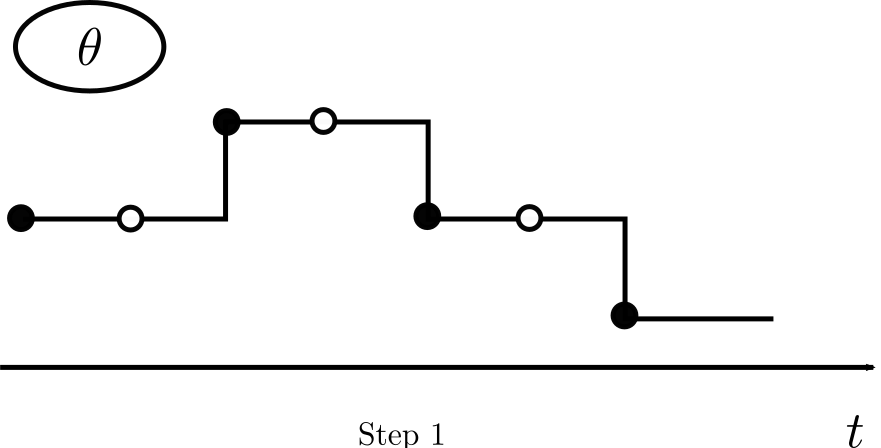
\includegraphics [width=0.70\textwidth, angle=0]{figs/plotn1.pdf}
    \vspace{-0 in}
  \end{minipage}
  \begin{minipage}[!hp]{0.45\linewidth}
  \centering
    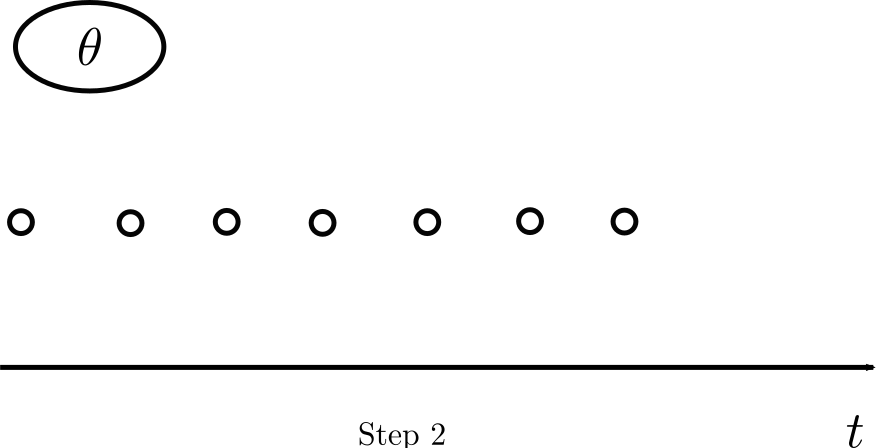
\includegraphics [width=0.70\textwidth, angle=0]{figs/plotn2.pdf}
    \vspace{-0 in}
  \end{minipage}
  \begin{minipage}[!hp]{0.45\linewidth}
  \centering
    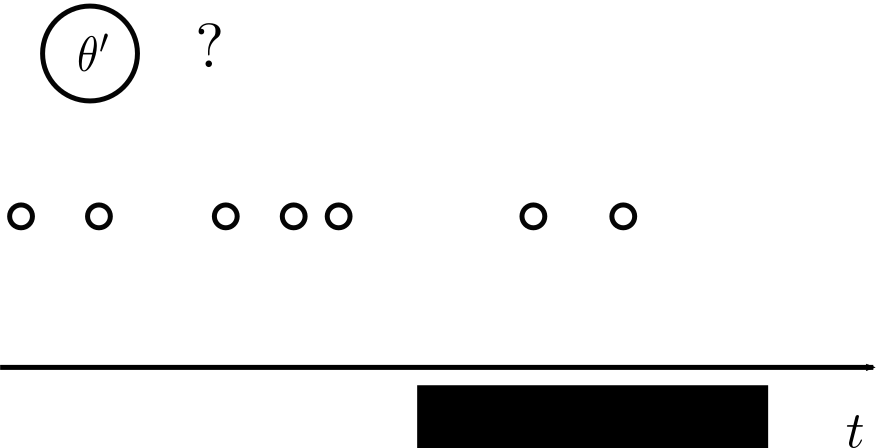
\includegraphics [width=0.70\textwidth, angle=0]{figs/plotn3.pdf}
    \vspace{-0 in}
  \end{minipage}
  \begin{minipage}[!hp]{0.45\linewidth}
  \centering
    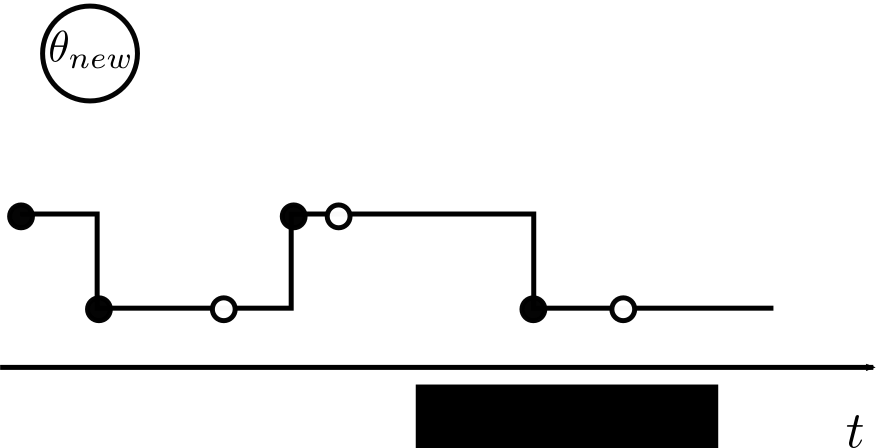
\includegraphics [width=0.70\textwidth, angle=0]{figs/plotn4.pdf}
    \vspace{-0 in}
  \end{minipage}
  \begin{minipage}[!hp]{0.45\linewidth}
  \centering
    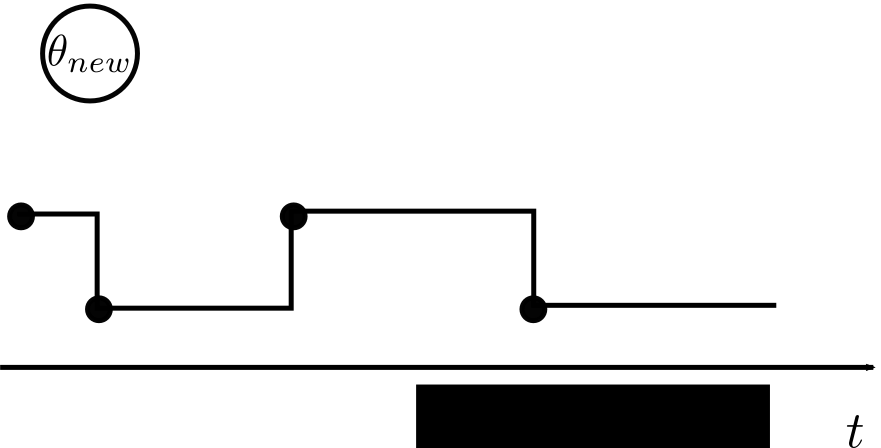
\includegraphics [width=0.70\textwidth, angle=0]{figs/plotn5.pdf}
    \vspace{-0 in}
  \end{minipage}
  \caption{\Naive\ MH-algorithm: Step 0 to 2: sample thinned events
  and discard state information to get a random grid. Step 3: 
propose a new parameter $\theta'$, and accept or reject by making
a forward pass on the grid. Steps 4 to 5: make a backward pass using
the accepted parameter and discard self-transitions to produce a new
trajectory.}
   \label{fig:naive_mh}
  \end{figure}

\subsection{Additional results}
In the following, we evaluate Python implementations of a number of algorithms, focusing our contribution, the symmetrized MH algorithm (algorithm~\ref{alg:MH_improved}), and as well as the \naive\ MH algorithm (algorithm~\ref{alg:MH_naive}).
%, which we plot \boqian{as yellow twodashed  lines}), 
%, plotted \sout{as dashed red lines}\boqian{as solid blue lines}
We evaluate different variants of these algorithms, corresponding to different uniformizing Poisson rates. % (i.e.\ different choices of $\kappa$, see section~\ref{sec:comments}). 
For \naive\ MH, we set $\Omega(\theta) = \kappa \max_s A_s(\theta) $ with $\kappa$  equal to $1.5, 2$ and $3$ (here $\kappa$ must be greater than $1$), 
%represented in our plots with circles, \sout{triangles} \boqian{square} and \sout{square} \boqian{triangles} symbols. 
while for symmetrized MH, where the uniformizing rate depends on both the current and proposed parameters, we consider the settings:
 $\Omega(\theta, \vartheta) = \kappa (\max A(\theta) + \max A(\vartheta))$ 
 ($\kappa = 1$ and $1.5$), and 
 %, plotted with \sout{triangles} \boqian{square} and \sout{square} \boqian{triangles}), and 
$\Omega(\theta, \vartheta) = 1.5 \max(\max A(\theta), \max A(\vartheta))$.
%($\kappa=1.5$, plotted with {circles}).  
We evaluate two other baselines: Gibbs sampling (Algorithm~\ref{alg:MJP_gibbs}), %plotted \sout{in blue} \boqian{as red long dashed lines} ), 
and particle MCMC~\citep[][see also section~\ref{sec:pmcmc} in the appendix]{Andrieu10}. 
%plotted \sout{in black} \boqian{as black dashed lines}. 
Gibbs sampling involves a uniformization step to update the MJP trajectory (step 1 in algorithm~\ref{alg:MJP_gibbs}), for which we use $\Omega(\theta,\vartheta) = \kappa \max_s A_s(\theta)$ for $\kappa=1.5,2,3$. 
%plotted with circles, \sout{triangles} \boqian{square} and \sout{square} \boqian{triangles}.  
Unless specified, our results were obtained from $100$ independent MCMC runs, each of $10000$ iterations.
We found particle MCMC to be more computationally intensive, and limited each run to $3000$ iterations, the number of particles being $5, 10$ and $20$.
For each run of each MCMC algorithm, we calculated the effective sample size (ESS) of the posterior samples of the MJP parameters using the R package \texttt{rcoda}~\citep{Rcoda2006}. 
This estimates the number of independent samples returned by the MCMC algorithm, and dividing this by the runtime of a simulation gives the ESS per unit time (ESS/sec). 
We used this to compare different samplers and different parameter settings. In the following we present the additional results.

  \begin{figure}[H]
  \centering
  \begin{minipage}[h!]{0.99\linewidth}
  \centering
    \includegraphics [width=0.24\textwidth, angle=0]{figs/new_whole_exp_figs/exp_alpha_dim3.pdf}
    \includegraphics [width=0.24\textwidth, angle=0]{figs/new_whole_exp_figs/exp_beta_dim3.pdf}
    \includegraphics [width=0.24\textwidth, angle=0]{figs/new_whole_exp_figs/exp_alpha_dim10.pdf}
    \includegraphics [width=0.24\textwidth, angle=0]{figs/new_whole_exp_figs/exp_beta_dim10.pdf}
  \end{minipage}

  \begin{minipage}[h!]{0.49\linewidth}
  \centering
    \includegraphics [width=0.49\textwidth, angle=0]{figs/new_whole_exp_figs/exp_alpha_dim5.pdf}
    \includegraphics [width=0.49\textwidth, angle=0]{figs/new_whole_exp_figs/exp_beta_dim5.pdf}
  \end{minipage}
  \begin{minipage}[!hp]{0.49\linewidth}
    \caption{ESS/sec for the synthetic model, The top left two panels are $\alpha$ and $\beta$ for 3 states, the bottom two, for 5 states, and the right two, for 10 states. Blue, yellow, red and black are the symmetrized MH, \naive\ MH, Gibbs and particle MCMC algorithm.  Squares, circles and trianges correspond to $\Omega(\theta,\vartheta)$ set to $(\max_s A_s(\theta) + \max_s A_s(\vartheta))$, $\max(\max_s A_s(\theta), \max_s A_s(\vartheta))$ and  $1.5(\max_s A_s(\theta) + \max_s A_s(\vartheta))$. And for PMCMC, they correspond to 10 particles, 5 particles and 15 particles.}
     \label{fig:ESS_EXP}
  \end{minipage}
  \end{figure}


  \begin{figure}[H]
%    \vspace{-.2in}
  \centering
  \begin{minipage}[!hp]{0.99\linewidth}
    \includegraphics [width=0.24\textwidth, angle=0]{figs/acc/EXP_D3alpha_k2.pdf}
    \includegraphics [width=0.24\textwidth, angle=0]{figs/acc/EXP_D5alpha_k2.pdf}
    \includegraphics [width=0.24\textwidth, angle=0]{figs/EXP_ks/exp_traceoMH_7_05_3_.pdf}
    \includegraphics [width=0.24\textwidth, angle=0]{figs/EXP_ks/exp_omhacf_7_05_3_.pdf}
  \end{minipage}
%  \begin{minipage}[!hp]{0.49\linewidth}
    \caption{Acceptance Rate for $\alpha$ in the synthetic model (Left two), the first being dimension 3, and the second,dimension 5. Blue square and yellow triangle curves are the symmetrized MH, and \naive\ MH  algorithm. The multiplicative factor is $2$. Trace and autocorrelation plots for \naive\ MH  (right two panels) for the synthetic model with $3$ states.}
     \label{fig:ACC_EXP}
%  \end{minipage}
  \end{figure}
%  \begin{figure}[H]

%  \centering

%  \begin{minipage}[!hp]{0.99\linewidth}
%  	\centering
 %   \includegraphics [width=0.3\textwidth, angle=0]{figs/acc/JCalpha_k2.pdf}
%	\hspace{.5in}
  %  \includegraphics [width=0.3\textwidth, angle=0]{figs/JC_ks/jc_hist_44_05_3_.pdf}
  %\end{minipage}
%  \begin{minipage}[!hp]{0.99\linewidth}
   % \caption{The left represents the acceptance rate for $\alpha$ in the JC69 model.  Blue and yellow curves represent symmetrized MH,and \naive\ MH  algorithm. The multiplicative factor is $2$.The right is histogram for the posterior samples($\alpha$) of the JC69 model, the red and blue curves are the Gibbs and symmetrized MH. The p value of the two sample-Kolmogorov Smirnov test is $ 0.97$.  }
  %   \label{fig:ACC_JC}
%  \end{minipage}
  %\end{figure}
  
  \begin{figure}[H]
%    \vspace{-.2in}
  \centering
%  \begin{minipage}[!hp]{0.99\linewidth}
 % \centering
  \begin{minipage}[!hp]{0.99\linewidth}
    \includegraphics [width=0.24\textwidth, angle=0]{figs/Q_ks/q_traceGBS_20_03_3_.pdf}
    \includegraphics [width=0.24\textwidth, angle=0]{figs/Q_ks/q_traceMH_20_03_3_.pdf}
    \includegraphics [width=0.24\textwidth, angle=0]{figs/Q_ks/q_gbsacf_20_03_3_.pdf}
    \includegraphics [width=0.24\textwidth, angle=0]{figs/Q_ks/q_mhacf_20_03_3_.pdf}
  \end{minipage}
  
%  \end{minipage}
%  \begin{minipage}[!hp]{0.99\linewidth}
%    \caption{The left is histogram for the posterior samples($\alpha$) of the immigration model with dimension 3, the red and blue curves are the Gibbs and symmetrized MH. The p value of the two sample-Kolmogorov Smirnov test is $ 0.978$. The middle and the right are trace plots for the posterior samples of the immigration model with dimension 3, the middle is for Gibbs and the right is for symmetrized MH}
\caption{Trace and autocorrelation plots for Gibbs (left two panels) and symmetrized MH (right two panels). All plots are for the immigration model with $3$ states.}
     \label{fig:TRACE_Q}
%  \end{minipage}
  \end{figure}
  
  \begin{figure}[H]
%    \vspace{-.2in}
  \centering
%  \begin{minipage}[!hp]{0.99\linewidth}
 % \centering
  \begin{minipage}[!hp]{0.99\linewidth}
    \includegraphics [width=0.24\textwidth, angle=0]{figs/QC_ks/qc_traceGBS_4_03_10_.pdf}
    \includegraphics [width=0.24\textwidth, angle=0]{figs/QC_ks/qc_traceMH_4_03_10_.pdf}
    \includegraphics [width=0.24\textwidth, angle=0]{figs/QC_ks/qc_gbsacf_4_03_10_.pdf}
    \includegraphics [width=0.24\textwidth, angle=0]{figs/QC_ks/qc_mhacf_4_03_10_.pdf}
  \end{minipage}

%  \end{minipage}
%  \begin{minipage}[!hp]{0.99\linewidth}
%    \caption{The left is histogram for the posterior samples($\alpha$) of the time-inhomogeneous immigration model with dimension 10, the red and blue curves are the Gibbs and symmetrized MH. The p value of the two sample-Kolmogorov Smirnov test is $ 0.7212$. The middle and the right are trace plots for the posterior samples of the time-inhomogeneous immigration model with dimension 10, the middle is for Gibbs and the right is for symmetrized MH}
\caption{Trace and autocorrelation plots for Gibbs (left two panels) and symmetrized MH (right two panels). All plots are for the time-inhomogeneous immigration model with $10$ states.}
 
     \label{fig:TRACE_CQ}
%  \end{minipage}
  \end{figure}


  \begin{figure}[H]
  \centering
  \begin{minipage}[h!]{0.99\linewidth}
  \centering
    \includegraphics [width=0.24\textwidth, angle=0]{figs/new_whole_exp_figs/q_alpha_dim3.pdf}
    \includegraphics [width=0.24\textwidth, angle=0]{figs/new_whole_exp_figs/q_beta_dim3.pdf}
    \includegraphics [width=0.24\textwidth, angle=0]{figs/new_whole_exp_figs/q_alpha_dim10.pdf}
    \includegraphics [width=0.24\textwidth, angle=0]{figs/new_whole_exp_figs/q_beta_dim10.pdf}
  \end{minipage}

  \begin{minipage}[h!]{0.49\linewidth}
  \centering
    \includegraphics [width=0.49\textwidth, angle=0]{figs/new_whole_exp_figs/q_alpha_dim5.pdf}
    \includegraphics [width=0.49\textwidth, angle=0]{figs/new_whole_exp_figs/q_beta_dim5.pdf}
  \end{minipage}
  \begin{minipage}[!hp]{0.49\linewidth}
    \caption{ESS/sec for the immigration model, The top left two panels are $\alpha$ and $\beta$ for 3 states, the bottom two, for 5 states, and the right two, for 10 states. Blue, yellow, and red are the symmetrized MH, \naive\ MH, Gibbs algorithm. Squares, circles and trianges correspond to $\Omega(\theta,\vartheta)$ set to $(\max_s A_s(\theta) + \max_s A_s(\vartheta))$, $\max(\max_s A_s(\theta), \max_s A_s(\vartheta))$ and  $1.5(\max_s A_s(\theta) + \max_s A_s(\vartheta))$.}
     \label{fig:ESS_Q}
  \end{minipage}
  \end{figure}


  \begin{figure}[H]
  \centering
  \begin{minipage}[h!]{0.99\linewidth}
  \centering
    \includegraphics [width=0.24\textwidth, angle=0]{figs/new_whole_exp_figs/cq_alpha_dim3.pdf}
    \includegraphics [width=0.24\textwidth, angle=0]{figs/new_whole_exp_figs/cq_beta_dim3.pdf}
    \includegraphics [width=0.24\textwidth, angle=0]{figs/new_whole_exp_figs/cq_alpha_dim10.pdf}
    \includegraphics [width=0.24\textwidth, angle=0]{figs/new_whole_exp_figs/cq_beta_dim10.pdf}
  \end{minipage}

  \begin{minipage}[h!]{0.49\linewidth}
  \centering
    \includegraphics [width=0.49\textwidth, angle=0]{figs/new_whole_exp_figs/cq_alpha_dim5.pdf}
    \includegraphics [width=0.49\textwidth, angle=0]{figs/new_whole_exp_figs/cq_beta_dim5.pdf}
  \end{minipage}
  \begin{minipage}[!hp]{0.49\linewidth}
    \caption{ESS/sec for the time-inhomogeneous immigration model, The top left two panels are $\alpha$ and $\beta$ for 3 states, the bottom two, for 5 states, and the right two, for 10 states. Blue, yellow, and red are the symmetrized MH, \naive\ MH, Gibbs algorithm. Squares, circles and trianges correspond to $\Omega(\theta,\vartheta)$ set to $(\max_s A_s(\theta) + \max_s A_s(\vartheta))$, $\max(\max_s A_s(\theta), \max_s A_s(\vartheta))$ and  $1.5(\max_s A_s(\theta) + \max_s A_s(\vartheta))$.}
     \label{fig:ESS_CQ}
  \end{minipage}
  \end{figure}




	\begin{figure}	
  \centering
  \begin{minipage}[!hp]{0.25\linewidth}
  \centering
    \includegraphics [width=0.99\textwidth, angle=0]{figs/new_whole_exp_figs/jc_alpha.pdf}
  \end{minipage}
  \begin{minipage}[!hp]{0.74\linewidth}
    \caption{ESS/sec for the JC immigration model, with 
      dimension 5. (Left, right) are $(\alpha, \beta)$. Blue, yellow and red curves are the symmetrized MH,
  \naive\ MH, and Gibbs algorithm.}
     \label{fig:ESS_pc_55}
  \end{minipage}


% \centering
% \begin{minipage}[!hp]{0.64\linewidth}
%   \hspace{.15in}
%   \includegraphics [width=0.44\textwidth, angle=0]{figs/ECOLI_beta.pdf}
%   \hspace{.15in}
%   \includegraphics [width=0.44\textwidth, angle=0]{figs/ECOLI_l2.pdf}
% \end{minipage}
%   \hspace{-.3in}
% \begin{minipage}[!hp]{0.05\linewidth}
%   \hspace{0in}
%   \end{minipage}
% \begin{minipage}[!hp]{0.33\linewidth}
%   \caption{ESS/sec for EColi data. The left column is for $\beta$, and the 
%   right is for $\lambda_2$. Red and blue curves are Gibbs algorithm and the symmetrized MH.}
% \end{minipage}
%    \label{fig:ECOLI_beta_l2}
  \end{figure}

  \begin{figure}[H]
  \centering
  \begin{minipage}[!hp]{0.99\linewidth}
    \includegraphics [width=0.24\textwidth, angle=0]{figs/acc/Q_D3alpha_k2.pdf}
    \includegraphics [width=0.24\textwidth, angle=0]{figs/acc/Q_D10alpha_k2.pdf}
    \includegraphics [width=0.24\textwidth, angle=0]{figs/acc/CQ_D3alpha_k2.pdf}
    \includegraphics [width=0.24\textwidth, angle=0]{figs/acc/CQ_D10alpha_k2.pdf}
  \end{minipage}
    \caption{Acceptance Rate for $\alpha$ in the immigration model (left two) and time-inhomogeneous immigration model (right two) , the left two being dimension 3, and the right,dimension 10 and the right two being dimension 3, and the right,dimension 10.  Blue square and yellow triangle curves represent symmetrized MH,
 and \naive\ MH  algorithm. The multiplicative factor is $2$. }
     \label{fig:ACC_Q}
  \end{figure}

%%%% Time-homog
%    \includegraphics [width=0.19\textwidth, angle=0]{figs/Q_ks/q_hist_20_03_3_.pdf}
%%%%%%%%

  \begin{figure}[H]
%    \vspace{-.2in}
  \centering

  \begin{minipage}[!hp]{0.49\linewidth}
    \includegraphics [width=0.49\textwidth, angle=0]{figs/QC_ks/qc_hist_4_03_10_.pdf}
    \includegraphics [width=0.49\textwidth, angle=0]{figs/Q_ks/q_hist_25_03_10_.pdf}
  \end{minipage}
  \begin{minipage}[!hp]{0.49\linewidth}
    \caption{Posterior $P(\alpha|X)$ from Gibbs (dashed line) and symmetrized MH (solid line) for the immigration model(Left), and time-inhomogeneous immigration model(right)}
     \label{fig:HIST_QCQ}
  \end{minipage}
  \end{figure}

  \begin{figure}[H]
%    \vspace{-.2in}
  \centering

  \begin{minipage}[!hp]{0.99\linewidth}
%	\centering
    \includegraphics [width=0.24\textwidth, angle=0]{figs/ecoli_ks/ecoli_alphahist_31_3_0_.pdf}
    \includegraphics [width=0.24\textwidth, angle=0]{figs/ecoli_ks/ecoli_l1hist_31_3_0_.pdf}
    \includegraphics [width=0.24\textwidth, angle=0]{figs/acc/ecolialpha_k2.pdf}

  \end{minipage}
%  \begin{minipage}[!hp]{0.99\linewidth}
    \caption{Posterior $P(\alpha|X)$ (left) and $P(\lambda_1|X)$ (middle) from Gibbs (dashed line) and symmetrized MH (solid line) for the E.\ Coli data. Acceptance Rate of $\alpha$ generated by the symmetrized MH algorithm for the E.\ Coli data . The multiplicative factor is $2$. }
     \label{fig:ACC_ECOLI}
%  \end{minipage}
  \end{figure}

\begin{proposition}
The a posteriori probability that the embedded Markov chain makes a
self-transition,
$P(V_i = V_{i + 1} | W, X, \theta, \vartheta) \ge \delta_1 > 0$,
for %$i = 0, 1, 2, ..., |W|$ and
any $\theta,\vartheta, W$.
\end{proposition}
\begin{proof}
  We use $k_0$ from assumption~\ref{asmp:unif_rate}
  to bound {\em a priori} self-transition probabilities:
  \begin{align*}
    P(V_{i + 1}=s|V_i=s,\theta,\vartheta) &= B_{ss}(\theta,\vartheta) =
    1 - \frac{A_{s}(\theta)}{\Omega(\theta, \vartheta)}
    \ge 1 - \frac{A_{s}(\theta)}{\Omega(\theta)} \ge 1-\frac{1}{k_0}.
    \intertext{  We then have}
%\mathbb{E}[\mathbb{I}_{\{V_i = V_{i + 1}\}} | W, X, \theta, \theta^*]
  P(V_i = V_{i + 1} | W, X, \theta, \vartheta) &= \sum_v P(V_i = V_{i + 1}
  = v | W, X, \theta, \vartheta)
 =\sum_v \frac{P(V_i = V_{i + 1} = v, X | W, \theta, \vartheta)}{P(X | W,
 \theta, \vartheta)} \\
&=\sum_v \frac{P(X | V_i = V_{i + 1} = v, W, \theta, \vartheta)P( V_i =
V_{i + 1} = v|W, \theta, \vartheta)}{P(X | W, \theta, \vartheta)}\\
& \geq \frac{\lb}{\ub}\sum_v P(V_i = V_{i + 1} = v | W, \theta, \vartheta)\\
&=  \frac{\lb}{\ub} \sum_v P(V_{i + 1} = v | V_i = v, W, \theta,\vartheta)P(V_i = v | \theta, \vartheta) \\
& \geq \frac{\lb}{\ub} (1-\frac{1}{k_0}) \assign \delta_1 > 0.
\end{align*}
\qed
\end{proof}



%\section{Geometrical ergodicity of the MH algorithm}~
As shown before, virtual jumps are sampled after uniformization procedure. Let's consider the redundant representation of the trajectory. $V = (v_0, v_1, v_2,..., v_n)$, $W = (w_1, w_2, w_3,..., w_n)$, where $v_i$ can be the same as $v_{i + 1}$. Denote $X$ as $(W, V, \theta)$. Also assume that noisy observations $Y = (Y_1, Y_2, ..., Y_k)$ are observed at some determined times $(t_1^{obs}, t_2^{obs}, ..., t_k^{obs})$. We will show that the chain of $X's$ is geometrically ergodic. Let $P$ be the transition kernel of the Markov chain $X_n$ generated by Algorithm 1. Let $\Pi(X)$ be the target distribution, which is the posterior distribution $P(X | Y)$. First, consider the following posterior distribution.
\begin{align*}
P(V | W, Y, \theta) &\propto  P(W, V | \theta) P(Y | W, V) p_0(\theta)\\
&= \nu_0(v_0)g_0(v_0; \theta)\prod_{i = 1}^n P(v_{i - 1}, v_i; \theta)g_i(v_i; \theta) p_0(\theta)\\
\end{align*}
\begin{align*}
g_i(v; \theta) &= \Omega(\theta) \exp(-(w_{i + 1} - w_i)\Omega(\theta)) \prod_{j: w_i < t_j^{obs} < w_{i + 1}} L_j(Y_j| v)\\
g_n(v; \theta) &= \exp(-(t_{end} - w_n)\Omega(\theta)) \prod_{j: w_n < t_j^{obs} < t_{end}} L_j(Y_j| v)\\
\end{align*}
Given the jumping times $W$, the state on the jumping times is a discrete time markov chain with $B(\theta)$ as transition matrix.
\begin{align*}
B(\theta) = I + \frac{A(\theta)}{\Omega(\theta)}\\
\end{align*}
The following is $n_0$ step transition probability.
\begin{align*}
B_{i - n_0 : i}(v_{i - n_0}, s_i = v; \theta) = \sum_{v_{i - n_0 + 1}, v_{i - n_0 + 2},...,v_{i - 1}} (\prod_{l = i - n_0 + 1}^{i - 1} B(v_{l - 1}, v_l; \theta))B(v_{i - 1}, v; \theta)\\
B_{i - n_0 : i}^{g}(v_{i - n_0}, s_i = v; \theta) = \sum_{v_{i - n_0 + 1}, v_{i - n_0 + 2},...,v_{i - 1}} (\prod_{l = i - n_0 + 1}^{i - 1} B(v_{l - 1}, v_l; \theta)g_l(v_l; \theta))B(v_{i - 1}, v; \theta)\\
\end{align*}
\begin{theorem}~
  Denote the state space as $S$ and the parameter space as $\Theta$, and assume that:\\
1. Exist an irreducible rate matrix $A^{min}$ such that $A(s, s';\theta) \geq A^{min}(s, s')$, for $\forall s \in S$ and $s' \in S$, where $s \neq s'$.\\
2. For $\forall \theta$, $\forall s$,  and the determined $\Omega(\theta)$, there exits an $\eta$ such that $\frac{A(s; \theta)}{\Omega(\theta)} \leq 1 - \eta$, where $A(s; \theta) = \sum_{s' \neq s} A(s, s';\theta)$.\\
3. $\exists \Omega^{max} < +\infty$, such that, $\forall \theta$, $\Omega(\theta) \leq \Omega^{max}$.\\
4. $\exists \kappa > 0$ such that the proposal distribution in MH step $q(\theta' | \theta) \geq \kappa q_0(\theta_0)$, where $q_0(\theta_0)$ is the prior distribution of $\theta$.\\
\indent Then the chain $X_n$ generated by Algorithm 1 is geometrically ergodic, i.e. there exist an constant $\gamma$ and a function $M(X)$ such that $L(Y | X) > 0$ and every m, $$\Vert P^m(X, \cdot) - \Pi(\cdot) \Vert_{tv} \leq \gamma^m M(X).$$
\end{theorem} 
\begin{lemma}~
   For a fixed $n_0$ , and $\forall$ $i$  such that $ n_0 \geq i \leq n - 1$, assume that\\
1. $\exists$  $ \xi > 0$, $B_{i - n_0: i}(v_{i - n_0}, v; \theta) \geq \xi$, $\forall$ $v_{i - n_0}, v \in S$.\\
2. $\exists$  $\eta > 0$, $B(v,v ; \theta) \geq \eta$, $\forall$, $v \in S$.\\
3. $\exists$  $g_l^{min} > 0$, $g_l^{max}$, such that $g_l^{min} \leq g_l(v; \theta) \leq g_l^{max}$, for $\forall$ $v \in S$, and $\forall$ $l \in [i - n_0 + 1, i]$\\ 
Then $\mathbb{P}(V_i = v | V_{i + 1} = v, W, \theta, Y) \geq \delta_i$ and $\delta_i = \xi\eta \prod_{l = i - n_0 + 1}^i \frac{g_l^{min}}{g_l^{max}}$.
\end{lemma}
\begin{proof}
  We condition on $V_{i - n_0} = v_{i - n_0}$ and we can get the following. 
\begin{align*}
\mathbb{P}(V_i = v | v_{i + 1} = v, V_{i - n_0} = v_{i - n_0} W, \theta, Y) &= \frac{\mathbb{P}(V_i = v | v_{i - 1} = v, V_{i - n_0}| W \theta, Y)}{\mathbb{P}(v_{i + 1} = v, V_{i - n_0}| W \theta, Y)} \\
&= \frac{B_{i - n_0: i}^g(v_{i - n_0}, v; \theta)g_i(v;\theta)B(v,v;\theta)}{\sum_{v'}B_{i - n_0: i}^g(v_{i - n_0}, v'; \theta)g_i(v';\theta)B(v',v;\theta)} \\
&\geq \frac{\prod_{l = i - n_0 + 1}^i g_l^{min}}{\prod_{l = i - n_0 + 1}^i g_l^{max}} \frac{B_{i - n_0: i}(v_{i - n_0}, v; \theta)B(v, v; \theta)}{\sum_{v'}B_{i - n_0: i}(v_{i - n_0}, v'; \theta)B(v', v; \theta)}\\
&\geq \xi \eta \prod_{l = i - n_0 + 1}^i \frac{g_l^{min}}{g_l^{max}}
\end{align*}
\end{proof}
\begin{lemma}~
 If the assumptions of Lemma 2 hold for $\forall$ $i \in [n_0, n - 1]$, then $\mathbb{E}[|J| | W, \theta, Y] \leq |W|  + 1- \sum_{i = n_0}^{|W| - 1} \delta_i$, where $J = \{i \in [1, n]: V_i \neq V_{i - 1}\} \cup \{ 0 \}$ for $\forall \theta \in \Theta$.
\end{lemma}
\begin{proof}
We notice that $|W| = n$. Apply lemma 2 to every $i \in [n_0, n - 1]$. We can get $\mathbb{P}(V_i = v| V_{i + 1}, W, \theta, Y) \geq \delta_i.$ Then $\mathbb{E} \mathbb{I}_{\{V_i \neq V_{i + 1} \}} = \mathbb{E}[\mathbb{P}(V_i \neq V_{i + 1}| V_{i + 1}, W, \theta, Y) | W, \theta, Y] \leq 1 - \delta_i$. Then we apply the naive upper bound $1$ for every $i < n_0$. Then $$\mathbb{E}[|J| | W, \theta, Y] = \mathbb{E}[1 + \sum_{i = 0}^{n - 1}\mathbb{I}_{\{V_i \neq V_{i + 1}\}}| W, \theta, Y] \leq n + 1 - \sum_{i = n_0} ^ {n - 1} \delta_i.$$
\end{proof}
\begin{proposition}
  (Drift Condition)  Under the assumptions of theorem 1, there exit   $0 < \delta < 1$ and $c < +\infty$ such that in one step of algorithm 1, $\mathbb{E} [|J(X')| |X] \leq (1 - \delta) |J(X)| + c$.
\end{proposition}
\begin{proof}
Assume the current state is $X = (V, W, \theta)$, where $V = (v_0, v_1, v_2,..., v_n)$, $W = (w_1, w_2, w_3,..., w_n)$. First we will show there exists a $n_0$, such that the assumptions of lemma 2 hold for this $n_0$. Let $B^{min} = I + \frac{A^{min}}{r^{max}}$. Because $A^{min}$ is irreducible, $B^{min}$ is irreducible too. So there exists $n_0 \in \mathbb{Z}^+$ and $\xi > 0$ such that $(B^{min})^{n_0}(v, v') \geq \xi$ for $\forall v, v' \in S$. So condition 1 of lemma 2 holds. Assumption 2 of Theorem 1 leads to condition 2 of lemma 2. \\
In the first step of algorithm 1, virtual jumps $U$ are sampled. And we get $W'$. $|U|$ is poisson distributed with rate $\int_{t_{start}}^{t_{end}}(\Omega(\theta) - A(X_t))dt \leq \Omega^{max}(t_{end} - t_{start})$. So $\mathbb{E}[|W'| | X] \leq |J(X)| + \Omega^{max}(t_{end} - t_{start})$.\\For condition 3 of lemma 2, the upper bound is uniform for all $l$. $g_l^{max} = \Omega^{max}$. For the lower bound, if $g_l(v; 
\theta)$ includes likelihood factors, then we simply use $0$ as lower bound. For the remaining, we have a uniform lower bound $g_l^{min} = \Omega^{min} \exp(\Omega^{max}(t_{end} - t_{start}))$, where $\Omega^{min} = \min_{v}\{ \sum_{v' \neq v} A(v, v')\}$. There are at most $k$  $g_l(v; \theta)$ which contains likelihood factors. If $g_l^{min} = 0$, then let $\delta_i = 0$ for $i \in [l, l + n_0 - 1]$. We also let $\delta_i = 0$ for $ i < n_0$. So there are at most $(k + 1) n_0$ indices $i$ such that $\delta_i = 0$. For at least $n - (k + 1)n_0$ indices such that $\delta_i = \xi \eta (\frac{g^{min}}{g^{max}})^{n_0} \triangleq \delta$ which is free of $\theta$.\\ 
Then apply lemma 3 using the $\delta_i$ we define earlier. $\mathbb{E}[|J'| W', \theta', Y] \leq |W'| + 1 - (|W'| - (k + 1) n_0) \delta \leq (1 - \delta) |W'| + ((k + 1)n_0\delta + 1)$\\
$$\mathbb{E}[J(X') | X] = \mathbb{E}[\mathbb{E}[J(X')| W'] | X] \leq (1- \delta)(|J(X)| + \Omega^{max}(t_{end} - t_{start})) + (k + 1)n_0\delta + 1.$$
\end{proof}
\begin{proposition}
  (Small set Condition)  The set $\{ X: |J(X)| \leq h \}$ is 1-small for every $h > 0$. I.e. there exits a probability measure $\Psi$ and a constant $\beta > 0$ such that $P(X, dX') \geq \beta \Psi(dX')$, where $|J(X)| \leq h$.
\end{proposition}
\begin{proof}
First choose a $V^\dagger = (v_1^\dagger, v_2^\dagger,..., v_k^\dagger)$ such that $\prod_{j = 1}^k L_j(Y_j|v_j^\dagger) \triangleq L^\dagger > 0$. Then define $V^\ast = (v_0^ \ast, v_1^\ast, ...,v_m^\ast)$ such that $V^\dagger$ is a sub-sequence of $V^\ast$, where $v_i^\ast \neq v_{i + 1}$. Also, embed $t^{obs} = (t_1^{obs}, t_2^{obs},..., t_k^{obs})$ in a longer time sequence $W^\ast = (w_1^\ast, w_2^\ast,...,w_m^\ast)$.\\
$$\nu_0(v_0^\ast) \prod_{i = 1} ^ {m - 1}B(v_i^\ast,v_{i + 1}^\ast; \theta) \geq \nu_0(v_0^\ast) \prod_{i = 1} ^ {m - 1} \frac{A^{min}(v_i^\ast,v_{i + 1}^\ast)}{\Omega^{max}} \triangleq \beta_2^\ast.$$
Define the regeneration measure $\Psi(dX')$ as follows.\\
$$W_i' \sim Unif(w_{i - 1}^\ast, w_i^\ast)$$ 
$$V_i' = v_i$$
$$\theta' \sim p_0(\cdot)$$
The random vector $(w_1', w_2',...,w_m')$ has the uniform distribution on the set $\tau = \{ (w_1, w_2,...,w_m)|w_{i - 1}^\ast \leq w_i\leq w_i^\ast\}$. There is another way in which algorithm 1 can be executed. $\Omega(\theta) - B(v; \theta) \geq \eta \Omega(\theta) \geq \eta \Omega^{min} \triangleq \epsilon$. In step 1, we independently sample two Poisson processes $U_0$ and $U_1$ with rates $\epsilon$ and $\Omega(\theta) - B(V_t; \theta)$. Let $U = U_0 \bigcup U_1$. Then $W' = J(X) \bigcup U$. $$\mathbb{P}(U_0 \in \tau) \triangleq \beta_0 > 0.$$
$$\mathbb{P}(U_1 = \varnothing) \geq \exp(-\Omega^{max}(t_{end} - t_{start})) \triangleq \beta_1 > 0.$$
In step 2 of algorithm 1, $\theta$ is updated under Metropolis Hasting scheme. First, $\theta'$ is proposed via the proposal kernel $q(\theta'| \theta)$, then $\theta'$ is accepted with probability $\alpha = 1 \wedge \frac{q(\theta | \theta')P(\theta'| W', Y)}{q(\theta' | \theta)P(\theta| W', Y)} \triangleq 1 \wedge \bar{\alpha}$. Assume $P(Y | V, W) \in [L_{min}, L_{max}]$
\begin{align*}
P(\theta, W', Y) &= \int p(V', \theta, W', Y) dV'\\
&= \int p_0(\theta)P(W, V | \theta)P(Y | V', W') dV'\\
&\in [L_{min}p_0(\theta)P(W'| \theta), L_{max}p_0(\theta)P(W'| \theta)]
\end{align*} 
We notice that $P(W' | \theta) = \Omega(\theta)^{|W'|}(t_{end} - t_{start})^{|W'|}\exp(-\Omega(\theta)(t_{end} - t_{start}))$
\begin{align*}
\bar{\alpha} &\geq \frac{q(\theta | \theta' )}{q(\theta' | \theta)} \frac{L_{min}}{L_{max}}\frac{P(W' | \theta')}{P(W'|\theta)}\frac{p_0(\theta)}{p_0(\theta)}\\
&\geq \frac{q(\theta| \theta')}{q(\theta' | \theta)}\frac{L_{min}}{L_{max}}(\frac{\Omega^{min}}{\Omega^{max}})^{|W'|}\exp(-\Omega^{max}(t_{end} - t_{start}))\frac{p_0(\theta')}{p_0(\theta)}\\
&\geq \kappa\frac{L_{min}}{L_{max}}(\frac{\Omega^{min}}{\Omega^{max}})^{|W'|}\exp(-\Omega^{max}(t_{end} - t_{start}))\frac{p_0(\theta')}{q(\theta' | \theta)}\\
&\triangleq \kappa C(|W'|)\frac{p_0(\theta')}{q(\theta' | \theta)}
\end{align*}
So for $\forall \theta' \in \Theta$, and given $W'$,
 \begin{align*}
&q(\theta' | \theta) \hat{\alpha} d\theta' \geq \kappa C(|W'|) p_0(\theta')d\theta'\\
&q(\theta' | \theta)  d\theta' \geq \kappa p_0(\theta')d\theta'\\
\end{align*}
So for $\forall \theta' \in \Theta$,  $\exists D(|W'|) = 1 \wedge C(|W'|) < +\infty$ such that $q(\theta' | \theta)\alpha d\theta' \geq D(|W'|)p_0(\theta')d\theta'$. We notice that $D(x)$ is decreasing with respect to $x$.\\
In step 2, FFBS is applied to sample a new trajectory given the jump times. We can use rejection sampling to do the same sampling $ V$ from $P(\cdot| W', \theta', Y)$ as follows.\\
(i) Simulate $V'$ with transition matrix $B(\cdot,\cdot;\theta')$ and initial distribution $\mu_0$.\\
(ii) Accept it with probability $\alpha= \frac{\mu_0(v_0')\prod_{i = 0}^{|W'| - 1}B(v_i', v_{i + 1}'; \theta)\prod_{i =0}^{|W'|}g_i(v_i'; \theta)}{\mu_0(v_0')\prod_{i = 0}^{|W'| - 1}B(v_i', v_{i + 1}';\theta) (\Omega(\theta))^{|W'| + 1}L_{max}} \geq \frac{(\Omega^{min})^{|W'| + 1}}{(\Omega^{max})^{|W'| + 1}L_{max}}$.\\
Suppose the current state is $X = (W, V, \theta)$ with $|J(X)| \leq h$ and the next state is $X' = (W', V', \theta)$. We define the following events\\
$(E_1)$: In step 1, we get $W' = J(X) \bigcup U_0$, and $U_0 \in \tau$. So $\mathbb{P}(E_1) \geq \beta_0 \beta_1 > 0$.\\
$(E_2)$: In step 2, we propose $\theta'$ and accept it. $\mathbb{P}(E_2) \geq D(m + h)p_0(\theta')d\theta'\triangleq \beta_2 p_0(\theta')d\theta'$, where $\beta_2 > 0$. \\
$(E_3)$: In step 3, all the jump times in $J(X)$ become virtual jump times. $\mathbb{P}(E_3) \geq \beta_2^\ast \eta^{|J(X)|} \geq \beta_2^\ast \eta^h \triangleq \beta_3 > 0$\\
$(E_4)$: given $E1$ -- $E3$, $V'$ is accepted. $\mathbb{P}(E_4) \geq (\frac{\Omega^{min}}{\Omega^{max}})^{m + h}\exp(-\Omega^{max}(t_{end} - t_{start})) \frac{L^\dagger}{L_{max}} \triangleq \beta_4$.\\
If $E_1$ -- $E_4$ happen, then a new trajectory $(W', V')$ is generated. It is independent with $X$. $p(W', V') = \Psi |_{(W,V)}(W', V')$.
So, $P(X, dX') \geq \beta_0\beta_1\beta_2\beta_3\beta_4 \Psi(dX')$.
\end{proof}
Theorem 1 directly follows from Propositions 4 and 5, according to Roberts and Rosenthal (2004).


\end{document}
